%!TEX encoding = UTF-8 Unicode
\documentclass[
    12pt,
    headings=small,
    parskip=half,           % Ersetzt manuelles setzten von parskip/parindent.
    bibliography=totoc,
    numbers=noenddot,       % Entfernt den letzten Punkt der Kapitelnummern.
    open=any,               % Kapitel kann auf jeder Seite beginnen.
   final                   % Entfernt alle todonotes und den Entwurfstempel.
    ]{scrreprt}

% ===================================Praeambel==================================

% Kodierung, Sprache, Patches {{{
\usepackage[T1]{fontenc}    % Ausgabekodierung; ermoeglicht Akzente und Umlaute
                            %  sowie korrekte Silbentrennung.
\usepackage[utf8]{inputenc} % Erlaub die direkte Eingabe spezieller Zeichen.
                            %  Utf8 muss die Eingabekodierung des Editors sein.
\usepackage[ngerman]{babel} % Deutsche Sprachanpassungen (z.B. Ueberschriften).
\usepackage{microtype}      % Optimale Randausrichtung und Skalierung.
\usepackage[
    babel,
    ]{csquotes}             % Korrekte Anfuehrungszeichen in der Literaturliste.
\usepackage{fixltx2e}       % Patches fuer LaTeX2e.
\usepackage{scrhack}        % Verhindert Warnungen mit aelteren Paketen.
% }}}

% Schriftarten {{{
\usepackage{mathptmx}       % Times. Package 'times.sty' is obsolete.
\usepackage[scaled=.92]{helvet}
\usepackage{courier}
% }}}

% Biblatex {{{
% \usepackage[
%     style=alphabetic,
%     backend=biber,
%     backref=true
%     ]{biblatex}             % Biblatex mit alphabetischem Style und biber.
% \bibliography{Literatur.bib}% Dateiname der bib-Datei.
% }}}

% Dokument- und Texteinstellungen {{{
\usepackage[
    a4paper,
    margin=2.54cm,
    marginparwidth=2.0cm,
    footskip=1.0cm
    ]{geometry}             % Ersetzt 'a4wide'.
\clubpenalty=10000          % Keine Einzelzeile am Beginn eines Paragraphen
                            %  (Schusterjungen).
\widowpenalty=10000         % Keine Einzelzeile am Ende eines Paragraphen
\displaywidowpenalty=10000  %  (Hurenkinder).
\usepackage{floatrow}       % Zentriert alle Floats.
\usepackage{ifdraft}        % Ermoeglicht \ifoptionfinal{true}{false}
\pagestyle{plain}           % keine Kopfzeilen
% \sloppy                     % großzügige Formatierungsweise
\deffootnote{1em}{1em}{\thefootnotemark.\ } % Verbessert Layout mehrzeiliger Fußnoten

\makeatletter
\AtBeginDocument{%
    \hypersetup{%
        pdftitle = {\@title},
        pdfauthor  = \@author,
    }
}
\makeatother
% }}}

% Weitere Pakete {{{
\usepackage{graphicx}       % Einfuegen von Graphiken.
\usepackage{tabu}           % Einfuegen von Tabellen.
\usepackage{multirow}       % Tabellenzeilen zusammenfassen.
\usepackage{multicol}       % Tabellenspalten zusammenfassen.
\usepackage{booktabs}       % Schönere Tabellen (\toprule\midrule\bottomrule).
\usepackage[nocut]{thmbox}  % Theorembox bspw. fuer Angreifermodell.
\usepackage{amsmath}        % Erweiterte Handhabung mathematischer Formeln.
\usepackage{amssymb}        % Erweiterte mathematische Symbole.
\usepackage{rotating}
\usepackage[
    printonlyused
    ]{acronym}              % Abkuerzungsverzeichnis.
\usepackage[
    colorinlistoftodos,
    textsize=tiny,          % Notizen und TODOs - mit der todonotes.sty von
    \ifoptionfinal{disable}{}%  Benjamin Kellermann ist das Package "changebar"
    ]{todonotes}            %  bereits integriert.
\usepackage[
    breaklinks,
    hidelinks,
    pdfdisplaydoctitle,
    pdfpagemode = {UseOutlines},
    pdfpagelabels,
    ]{hyperref}             % Sprungmarken im PDF. Laed das URL Paket.
    \urlstyle{rm}           % Entfernt die Formattierung von URLs.
\usepackage{breakurl}
\def\UrlBreaks{\do\/\do-}
\usepackage{listings}       % Spezielle Umgebung für...
    \lstset{                %  ...Quelltextformatierung.
        language=C,
        breaklines=true,
        breakatwhitespace=true,
        frame=L,
        captionpos=b,
        xleftmargin=6ex,
        tabsize=4,
        numbers=left,
        numberstyle=\ttfamily\footnotesize,
        basicstyle=\ttfamily\footnotesize,
        keywordstyle=\bfseries\color{green!50!black},
        commentstyle=\itshape\color{magenta!90!black},
        identifierstyle=\ttfamily,
        stringstyle=\color{orange!90!black},
        showstringspaces=false,
        }
% }}}

% ===================================Dokument===================================

\usepackage{url}
\usepackage[linewidth=1pt]{mdframed}

% Commands for protocol messages etc.

% Protocols
\newcommand{\recordprotocol}			{Record-Protokoll}
\newcommand{\handshakeprotocol}			{Handshake-Protokoll}
\newcommand{\alertprotocol}				{Alert-Protokoll}
\newcommand{\changecipherspecprotocol}	{ChangeCipherSpec-Protokoll}
\newcommand{\applicationdataprotocol}	{ApplicationData-Protokoll}

% Handshake messages
\newcommand{\hellorequest}			{HelloRequest}
\newcommand{\clienthello}			{ClientHello}
\newcommand{\serverhello}			{ServerHello}
\newcommand{\servercertificate}		{ServerCertificate}
\newcommand{\serverkeyexchange}		{ServerKeyExchange}
\newcommand{\certificaterequest}	{CertificateRequest}
\newcommand{\serverhellodone}		{ServerHelloDone}
\newcommand{\clientcertificate}		{ClientCertificate}
\newcommand{\clientkeyexchange}		{ClientKeyExchange}
\newcommand{\certificateverify}		{CertificateVerify}
\newcommand{\changecipherspec}		{ChangeCipherSpec}
\newcommand{\finished}				{Finished}

% Misc
\newcommand{\badrecordmac}			{bad\_record\_mac}
\newcommand{\badcertificate}		{bad\_certificate}
\newcommand{\decryptionfailed}		{decryption\_failed}

\newcommand{\mastersecret}			{MasterSecret}
\newcommand{\premastersecret}		{PreMasterSecret}

\newcommand{\ciphersuite}{Cipher-Suite}
\newcommand{\ciphersuites}{Cipher-Suites}

% Helper
\newcommand{\datafield}[1]{\texttt{#1}} %{\textbf{\texttt{#1}}}
\newcommand{\monospace}[1]{\texttt{#1}}
\newcommand{\inquotes}[1]{\glqq#1\grqq}


% Labelformat
%\label{fig_XYZ} Abbildungen
%\label{sec_XYZ} Abschnitte
%\label{cha_XYZ} Kapitel

\title{Funktionsweise, Angriffe und Abwehrmechanismen von SSL/TLS}
\author{Tom Petersen}
% \date{01.01.2015} % falls ein bestimmter Tag eingesetzt werden soll, einfach diese Zeile aktivieren

\begin{document}

\thispagestyle{empty}
% \addcontentsline{toc}{chapter}{Muster des Deckblatts}
\begin{titlepage}% {{{
\begin{center}\Large
	Universität Hamburg \par
	Fachbereich Informatik
	\vfill
	Bachelorarbeit
	\vfill
	\makeatletter
	{\Large\textsf{\textbf{\@title}}\par}
	\makeatother
	\vfill
	vorgelegt von
	\par\bigskip
	\makeatletter
	{\@author} \par
	\makeatother
	geb. am 13. Dezember 1990 in Hannover \par
	Matrikelnummer 6359640 \par
	Studiengang Informatik
	\vfill
	\makeatletter
	eingereicht am {\@date}
	\makeatother
	\vfill
	Betreuer: Dipl.-Inf. Ephraim Zimmer\par
	Erstgutachter: Prof. Dr.-Ing. Hannes Federrath \par
	Zweitgutachter: Dr. Dominik Herrmann
\end{center}
\ifoptionfinal{}{
\begin{tikzpicture}[remember picture, overlay]
    \node[draw, red, font=\ttfamily\bfseries\Huge, xshift=-50mm, yshift=238mm,
        rotate=10, text centered, text width=8cm, very thick, rounded
        corners=4mm] at (current page.south) {Entwurf vom \today};
\end{tikzpicture}}
\end{titlepage}% }}}

\chapter*{Aufgabenstellung}

Die Protokollfamilie SSL/TLS umfasst Techniken zum Schutz von Kommunikationsdaten in IP-basierten Netzen. Ihre weite Verbreitung und Wichtigkeit für die IT-Sicherheit ist historisch gewachsen, und ihr Einsatz erstreckt sich über mittlerweile weit mehr Protokolle der Anwendungsschicht, als nur das ursprünglich anvisierte HTTP. Diese weite Verbreitung hat zwei wesentliche Konsequenzen. Zum einen wurden sowohl die Spezifikation der Protokollfamilie als auch praktische Implementierungen von SSL/TLS Gegenstand zahlreicher Angriffe. Zum zweiten sind ein grundlegendes Verständnis der Funktionsweise von SSL/TLS und der erwähnten Angriffe obligatorisch bei der Entwicklung und Implementierung von verteilter Software, Internetdiensten und Protokollimplementierungen auf der Anwendungsschicht, die mittels SSL/TLS abgesichert werden sollen. 

In dieser Bachelorarbeit soll unter Einbeziehung aktueller Entwicklungen und Forschungsergebnisse die Funktionsweise von SSL/TLS, bedeutende Angriffe auf diese Protokollfamilie sowie daraus erarbeitete Anpassungen der Protokollspezifikation und Abwehrmechanismen erläutert und speziell für den Einsatz in der Hochschullehre aufbereitet werden. Darüber hinaus soll ein modular aufgebautes Tool zur Veranschaulichung der SSL/TLS-Funktionsweise sowie deren Angriffe und Abwehrmechanismen entwickelt und prototypisch umgesetzt werden. Der Fokus des Tools liegt in der Demonstration von SSL/TLS und dessen Schwächen mit beliebiger Verständnisvertiefung, sollte allerdings auch um weitere IT-Sicherheitsprotokolle erweiterbar sein.

\chapter*{Zusammenfassung}

\todo{Abstract schreiben}

Für den eiligen Leser sollen auf etwa einer halben, maximal einer Seite die wichtigsten Inhalte, Erkenntnisse, Neuerungen bzw. Ergebnisse der Arbeit beschrieben werden.

Durch eine solche Zusammenfassung (im engl. auch Abstract genannt) am Anfang der Arbeit wird die Arbeit deutlich aufgewertet. Hier sollte vermittelt werden, warum der Leser die Arbeit lesen sollte.

\setcounter{tocdepth}{1}
\tableofcontents

\chapter{Einleitung}

%Warum diese Arbeit (Motivation), Thema eingrenzen \& Ziel der BA, Methodik

%Thematische Hinführung
TLS ist eines der bedeutendsten Sicherheitsprotokolle, das heute verwendet wird. Viele andere Protokolle setzen darauf auf, um ihre Kommunikation abzusichern. Aufgrund seiner Bedeutung wurde es im Laufe seiner Entwicklung oft untersucht und angegriffen. Dabei sind viele einfache und elegante Angriffe gefunden worden, die zeigen, wie wirksam die kleinsten Schwächen in Protokollen ausgenutzt werden können. Ebenso bieten Änderungen in der TLS-Spezifikation auch Beispiele für erfolgreiche Gegenmaßnahmen, die diese Angriffe verhindern.

%...

%inhaltlichen und welche methodischen Aspekte
In dieser Arbeit soll das TLS-Protokoll auf seine Eignung für den Einsatz in der Hochschullehre überprüft und dafür aufbereitet werden. 
Neben einer ausführlichen Betrachtung der Funktionsweise von TLS und existierenden Angriffen gegen die Protokollfamilie werden Empfehlungen für die Nutzung in der Lehre herausgearbeitet. Außerdem wird eine interaktive Anwendung entwickelt, die die Protokollabläufen während einer TLS-Verbindung simuliert und damit ein vertieftes Verständnis von TLS unterstützt.

%Kapitelweises Vorgehen erläutern
In Kapitel \ref{cha_cryptographic_techniques} werden in TLS zur Anwendung kommende kryptographische Verfahren eingeführt und die in dieser Arbeit verwendete Notation erläutert. \\
Der erste Teil der Arbeit behandelt die Grundlagen von TLS und entdeckter Angriffe. Das Kapitel \ref{sec_tls_overview} beschäftigt sich ausführlich mit der Funktionsweise von TLS anhand der aktuellen Protokollversion TLS 1.2. In Kapitel \ref{cha_attacks} wird auf bisher entdeckte Angriffe gegen SSL und TLS und getroffene Abwehrmechanismen eingegangen.\\
Im zweiten Teil der Arbeit geht es um den Einsatz von TLS in der Hochschullehre. Dazu werden in Kapitel \ref{cha_tls_teaching} Schwerpunkte für die Lehre herausgearbeitet, die am Beispiel von TLS erläutert werden können. Außerdem werden didaktische Grundlagen für die im Rahmen dieser Bachelorarbeit entwickelte Protokollsimulation gelegt. In Kapitel \ref{cha_implementation} wird dann der Aufbau der Anwendung und der Erweiterung um TLS beschrieben.

%Hauptsächlich verwendete Literatur?
Ein Großteil dieser Arbeit stützt sich direkt auf die TLS 1.2-Spezifikation in \cite{tls12}. Für die Grundlagen zu verwendeten kryptographischen Verfahren wurden \cite{Schneier2006} und \cite{ferguson10} zu Hilfe genommen. 
%-> Schneier, Schneier \& Ferguson als Grundlagenwerke zu Krypto
%-> TLS-Spezifikation für Tls-Kapitel und als Grundlage für die Implementation
%-> Angriffe: jeweilige Paper
%-> Dings, Dings und Dings als Grundlage für didaktische Empfehlungen
%-> Evtl. Design Patterns als Unterstützung für Implementierung

\chapter{SSL und TLS - ein Überblick}

SSL (Secure Socket Layer) bzw. TLS\footnote{Im weiteren Verlauf dieser Arbeit wird der Einfachheit halber lediglich von TLS gesprochen. Bei etwaigen Unterschieden wird explizit auf diese eingegangen.} (Transport Layer Security) ist ein zustandsbehaftetes Protokoll, das auf dem TCP-Protokoll\footnote{DTLS (Datagram Transport Layer Security) ist ein auf TLS basierendes Protokoll, dass auf UDP aufsetzt.} der Transportschicht des TCP/IP-Protokollstapels aufbaut. 

Hauptaufgaben von TLS sind Authentifikation der Kommunikationspartner, Verschlüsselung der Kommunikation sowie die Sicherstellung der Integrität der übertragenen Nachrichten (\cite{meyer14}). Dazu läuft die Kommunikation über TLS in zwei Phasen ab: Zu Beginn wird eine sichere Verbindung durch Festlegung der verwendeten kryptographischen Verfahren und des Schlüsselmaterials hergestellt. Danach können Daten transparent für Anwendungen und auf TLS aufbauende Protokolle über diese Verbindung gesendet werden.\\
Einige Beispiele für solche Protokolle und Anwendungen der Anwendungsschicht, die TLS nutzen, sind:
\begin{description}
\item[HTTPS] für die Datenübertragung, zumeist für die Auslieferung von Webseiten genutzt. 
\item[FTPS] für die Dateiübertragung.
\item[SMTP] für das Senden und Weiterleiten von E-Mails (als SMTPS oder per STARTTLS\footnote{\label{fn_starttls}SMTPS/IMAPS/POP3S beginnen die TLS-Verbindung bereits direkt nach dem Verbindungsaufbau und laufen, um dieses Verhalten zu erzwingen, über einen anderen Serverport. STARTTLS ist ein Kommando, das nach Verbindungsaufbau gesendet werden kann, um eine TLS-Verbindung zu initiieren.}).
\item[IMAP] für den Zugriff auf E-Mails auf Mailservern (als IMAPS oder per STARTTLS\textsuperscript{\ref{fn_starttls}}).
\item[POP3] für den Abruf von E-Mails von Mailservern (als POP3S oder per STARTTLS\textsuperscript{\ref{fn_starttls}}).
\item[OpenVPN,] eine verbreitete VPN-Software.
\end{description}

SSL wurde von der Firma Netscape entwickelt und zuerst in ihrem Browser, dem Netscape Navigator, verwendet. Nach mehreren neuen Protokollversionen und nachdem es starke Verbreitung gefunden hatte, wurde es durch die IETF als TLS 1.0 standardisiert (TLS 1.0 entspricht SSL 3.1). Aktuell ist die TLS-Version 1.2 und an Version 1.3 wird gearbeitet.\\
Inzwischen ist TLS laut \cite{schmeh09} das "`gegenwärtig meistverwendete Verschlüsselungsprotokoll im Internet"'. Gründe hierfür sind dem Autor zufolge insbesondere die leichte Integrierbarkeit in bestehende Strukturen, die "`[im Gegensatz zu IPSec] deutlich schnörkelloser[e] und einfacher[e]"' Protokollspezifikation und auch die marktreife Verfügbarkeit in den frühen 90er Jahren.

\section{Implementierungen}

Kurz sollen hier auch noch bestehende Implementierungen von SSL/TLS erwähnt werden, auch wenn der Fokus der Arbeit auf der Protokollspezifikation selber liegt.

Die meistgenutzte Implementierung, die unter anderem auch im häufig verwendeten Apache-Webserver zum Einsatz kommt, ist OpenSSL, eine Open-Source-Implementierung in C. In Produkten von Microsoft wird die Bibliothek SChannel, in Apple-Anwendungen Secure Transport und in Google Chrome und Mozilla-Produkten NSS verwendet. Auch manche Programmiersprachen bringen eigene Implementierungen mit. Ein Beispiel hierfür ist die Java Secure Socket Extension(JSSE) in Java.

Zusätzlich gibt es viele weitere seltener genutzte Implementierungen wie GnuTLS, PolarSSL, LibreSSL oder Amazon s2n, die vollständig neu entwickelt wurden oder als Forks bestehender Implementierungen entstanden sind.

Viele Angriffe auf TLS-gesicherte Verbindungen, die bekannt geworden sind, waren Angriffe auf Implementierungen und nicht auf die Protokollspezifikation selbst (auf diese zweite Art von Angriffen wird in Kapitel \ref{cha_attacks} eingegangen). Ein Beispiel ist der Heartbleed\footnote{http://heartbleed.com/} getaufte Bug in OpenSSL, der es wegen eines Programmierfehlers ermöglichte, Speicherinhalte des Servers auszulesen. Auf solche Angriffe, die lediglich einzelne Implementierungen betreffen, soll im Rahmen dieser Arbeit nicht weiter eingegangen werden.

Eine gelungene Übersicht über bestehende Implementierungen, die tiefer ins Detail geht, ist in \cite{meyer14} zu finden.
%https://en.wikipedia.org/wiki/Comparison_of_TLS_implementations

\chapter{Nach Besprechung mit Ephraim: Einführung}

In diesem Kapitel soll ein kurzer Überblick über die im Laufe der Arbeit relevanten kryptographischen Verfahren gegeben werden, sowie die verwendete Notation vorgestellt werden.

\section{Genutzte Verfahren(?)}

UML

Automat



\section{Kryptographische Verfahren}

\todo{Nette Bildchen}

\subsection{Symmetrische Kryptographie}

Symmetrische Kryptographie beschreibt Verfahren, bei denen bei der Ver- und Entschlüsselung der gleiche (oder ein aus dem anderen Schlüssel leicht berechenbarer) Schlüssel verwendet wird. Vor einer Kommunikation müssen beide Kommunikationspartner im Besitz dieses Schlüssels sein, ihn also über einen sicheren Kanal ausgetauscht haben.\\
Es gilt:
\[E_K(M)=C\] 
\[D_K(C)=M\] 
Hierbei steht \(M\) für die Nachricht, \(K\) für den Schlüssel, der verwendet wird, \(C\) für den Chiffretext und \(E\) bzw. \(D\) für die Ver- bzw. Entschlüsselung.

Symmetrischen Chiffren lassen sich in Strom- und Blockchiffren unterteilen.

\subsubsection{Stromchiffren}

Stromchiffren sind symmetrische Verschlüsselungsalgorithmen, die Klartexte bitweise zu Chiffretexten konvertieren. Die einfachste Möglichkeit ist die XOR-Verknüpfung der Klartextbits mit einem schlüsselabhängig generierten Bitstrom (Schlüsselstrom). Durch erneute XOR-Verknüpfung mit dem selben Schlüsselstrom auf der Empfängerseite lässt sich der Klartext zurückerhalten. Ein Beispiel für eine heute verwendete Stromchiffre ist RC4 \cite{Schneier2006}.

\subsubsection{Blockchiffren}

Bei Blockchiffren handelt es sich um symmetrische Verschlüsselungsalgorithmen, die Nachrichten in Blöcken fester Größe verschlüsseln.  Beispiele für heute verwendete Blockchiffren sind AES oder Twofish.

Da eine Blockchiffre immer nur einen Block verschlüsseln kann, muss festgelegt werden, wie mit mehreren Blöcken verfahren werden soll. Die Beschreibung eines solchen Verfahrens wird Betriebsmodus genannt.

Der einfachste Modus ist der ECB-Modus (Electronic Codebook). In diesem Modus wird jeder Block einzeln und unabhängig von anderen Blöcken verschlüsselt. Dieser Modus ist als unsicher zu betrachten, da die Verschlüsselung gleicher Klartextblöcke mit gleichem Schlüssel immer zu dem gleichen Chiffretextblock führt und ein Angreifer außerdem nach Belieben einzelne Blöcke entfernen, hinzufügen oder austauschen kann, ohne dass dies zwingend bemerkt wird.

Ein Beispiel für einen sichereren Modus ist CBC (Cipher Block Chaining). Hierbei erfolgt eine XOR-Verknüpfung des zuletzt erhaltenen Chiffretextblocks mit dem nächsten Klartextblock vor seiner Verschlüsselung. Zusätzlich wird für den ersten Klartextblock ein zusätzlicher, zufällig gewählter Block, der sogenannte Initialisierungsvektor (IV), benötigt \cite{Schneier2006}.

Einen Sonderfall stellen die AEAD-Chiffren (Authenticated Encryption with Associated Data) dar. Hierbei handelt es sich um Betriebsmodi, die ohne zusätzlichen Message Authentication Code (siehe Abschnitt \ref{sec_mac}) Authentizität und Integrität bereitstellen. Beispiele für solche Modi sind CCM (Counter with CBC-MAC) oder GCM (Galois/Counter Mode). 

\subsection{Asymmetrische Kryptographie}

Asymmetrische Kryptographie (oftmals auch Public-Key-Kryptographie) beschreibt Verfahren, bei denen bei der Ver- und Entschlüsselung verschiedene Schlüssel verwendet werden. Diese lassen sich nicht aus dem jeweils anderen Schlüssel berechnen. Daher kann ein Empfänger seinen öffentlichen Schlüssel bekanntgeben. Nachrichten, die mit diesem Schlüssel verschlüsselt werden, kann ein Angreifer trotzdem nicht lesen, da nur der Empfänger im Besitz seines geheimen Schlüssels ist. Es gilt: 
\[E_{K_{\text{public}}}(M)=C\] 
\[D_{K_{\text{private}}}(C)=M\] 
Hierbei steht \(K_{\text{public}}\) für den öffentlichen und \(K_{\text{private}}\) für den geheimen Schlüssel des Empfängers.

Durch asymmetrische Kryptographie lässt sich das bei symmetrischen Algorithmen bestehende Problem des Schlüsselaustauschs durch Veröffentlichung des öffentlichen Schlüssels leicht lösen. Das Problem, das hierbei entsteht, ist jedoch die Identität des Besitzers eines öffentlichen Schlüssels sicherzustellen. 

Ein Beispiel für einen asymmetrischen Algorithmus ist das RSA-Verfahren \cite{Schneier2006}.

\subsection{Diffie-Hellmann-Verfahren}

Das Diffie-Hellmann-Verfahren (DH-Verfahren) ist ein ebenfalls auf geheimen und öffentlichen Schlüssel basierendes Verfahren, das jedoch nicht der Ver- bzw. Entschlüsselung, sondern lediglich der Schlüsselvereinbarung dient. Es ermöglicht zwei Kommunikationspartnern einen Schlüssel zu erzeugen, ohne dass dieser direkt gesendet werden muss \cite{Schneier2006}. 

\subsection{Hashfunktion}

Eine Hashfunktion ist eine Funktion, die eine Eingabe variabler Länge auf einen String fester Länge abbildet.

In der Kryptographie werden insbesondere Einweg-Hashfunktionen eingesetzt. Bei dieser Art von Hashfunktionen ist es leicht, aus einer Eingabe den Hashwert zu berechnen, jedoch sehr schwer, zu einem gegebenen Hashwert eine Eingabe zu finden, die auf diesen Wert abgebildet wird \cite{Schneier2006}. Beispiele für heute verwendete Hashfunktionen sind MD5 und SHA256.

\subsection{Message Authentication Code}

\label{sec_mac}

Ein Message Authentication Code (MAC) ist ein Verfahren, das der Authentizität und dem Schutz der Integrität einer Nachricht dient. Dazu wird vom Sender aus einem geheimen Schlüssel \(K\) und der Nachricht \(M\) eine Art Prüfsumme generiert und zusammen mit der Nachricht versendet. Der Empfänger kann den MAC überprüfen, wenn er im Besitz des gleichen geheimen Schlüssels ist, und so sicherstellen, dass die Nachricht nicht verändert wurde. Ein Beispiel für einen solchen MAC ist der auch in TLS verwendete HMAC \cite{Schneier2006, ferguson10}.

\section{Verwendete Notationen}

In den folgenden Kapiteln werden die unten stehenden Notationen verwendet. Aus anderen Veröffentlichungen entnommene Passagen wurden teilweise geringfügig angepasst, um diesen Notationen zu folgen.

\(|B|\) steht für die Länge einer Zeichenkette B

\(A \oplus B\) entspricht der bitweisen XOR-Verknüpfung zweier Zeichenketten A und B

\(A + B\) steht für die Konkatenation zweier Zeichenketten A und B

\(0x\dots\) entspricht einer Zahl im hexadezimalen System



\lstset{style=tls}

\chapter{Funktionsweise von TLS}
\label{sec_tls_overview}

SSL (Secure Socket Layer) bzw. TLS (Transport Layer Security) ist ein zustandsbehaftetes Protokoll, das auf dem TCP-Protokoll\footnote{
	Es existiert auch noch DTLS (Datagram Transport Layer Security), ein zu TLS ähnliches Protokoll, das auf UDP aufsetzt. Dieses Protokoll wird im Rahmen dieser Arbeit jedoch nicht weiter behandelt.
} der Transportschicht des ISO/OSI-Schichtenmodells aufbaut. 

Hauptaufgaben von TLS sind Authentifikation der Kommunikationspartner, Verschlüsselung der Kommunikation sowie die Sicherstellung der Integrität der übertragenen Nachrichten \cite{meyer14}. Dazu läuft die Kommunikation über TLS in zwei Phasen ab: Zu Beginn wird eine sichere Verbindung durch Festlegung der verwendeten kryptographischen Verfahren und des Schlüsselmaterials hergestellt. Danach können Daten transparent für Anwendungen und auf TLS aufbauende Protokolle über diese Verbindung gesendet werden.\\
Einige Beispiele für solche Protokolle und Anwendungen der Anwendungsschicht, die TLS nutzen, sind:
\begin{description}
\item[HTTPS] für die Datenübertragung, zumeist für die Auslieferung von Webseiten genutzt. 
\item[FTPS] für die Dateiübertragung.
\item[SMTP] für das Senden und Weiterleiten von E-Mails (als SMTPS oder per STARTTLS\footnote{\label{fn_starttls}
	SMTPS/IMAPS/POP3S beginnen die TLS-Verbindung bereits direkt nach dem Verbindungsaufbau und laufen über einen anderen Serverport, um dieses Verhalten zu erzwingen. STARTTLS ist ein Kommando, das nach Verbindungsaufbau gesendet werden kann, um eine TLS-Verbindung zu initiieren.}).
\item[IMAP] für den Zugriff auf E-Mails auf Mailservern (als IMAPS oder per STARTTLS\textsuperscript{\ref{fn_starttls}}).
\item[POP3] für den Abruf von E-Mails von Mailservern (als POP3S oder per STARTTLS\textsuperscript{\ref{fn_starttls}}).
\item[OpenVPN,] eine verbreitete VPN-Software.
\end{description}

SSL wurde von der Firma Netscape entwickelt und zuerst in ihrem Browser, dem Netscape Navigator, verwendet. Nach mehreren neuen Protokollversionen und nachdem es starke Verbreitung gefunden hatte, wurde es durch die IETF als TLS 1.0 standardisiert (TLS 1.0 entspricht SSL 3.1). Aktuell ist die TLS-Version 1.2 und an Version 1.3 wird gearbeitet\footnote{
	Im weiteren Verlauf dieser Arbeit wird der Einfachheit halber lediglich von TLS gesprochen. Bei etwaigen Unterschieden zwischen den Protokollversionen wird explizit auf diese eingegangen.
}.\\
Inzwischen ist TLS das \inquotes{gegenwärtig meistverwendete Verschlüsselungsprotokoll im Internet}\cite{schmeh09}. Gründe hierfür sind dem Autor zufolge insbesondere die leichte Integrierbarkeit in bestehende Strukturen, die \inquotes{[im Gegensatz zu IPSec] deutlich schnörkelloser[e] und einfacher[e]} Protokollspezifikation und auch die marktreife Verfügbarkeit in den frühen 90er Jahren.

In den folgenden Abschnitten wird die Funktionsweise von TLS anhand der aktuellen Version 1.2 im Detail betrachtet. Dazu wird zunächst ein Überblick über die Teilprotokolle gegeben und diese anschließend genauer beleuchtet. Abschließend werden kurz Unterschiede zu anderen Protokollversionen betrachtet und auf bestehende Implementierungen der Spezifikation eingegangen.

\section{Teilprotokolle}

Die Informationen in diesem und den folgenden Abschnitt stammen überwiegend aus der TLS 1.2-Spezifikation \cite{tls12}. Für einen ersten Überblick wurde \cite{eckert13} genutzt.

TLS besteht aus zwei Schichten. Eine Übersicht über diese Schichten bietet Abbildung \ref{fig_tls_protocol_hierarchie}.\\
In der oberen Schicht sind vier Teilprotokolle spezifiziert: das \handshakeprotocol{}, das zum Aushandeln von kryptographischen Algorithmen und zur Vereinbarung von Schlüsselmaterial dient, das \changecipherspecprotocol{}, das den Beginn der Nutzung dieser Algorithmen regelt, das \alertprotocol{}, das das Versenden von Fehlerinformationen in der Verbindung übernimmt und das \applicationdataprotocol{}, das für den Austausch von Anwendungsdaten genutzt wird. Auf diese Protokolle soll später eingegangen werden.\\ 
In der unteren Schicht befindet sich das \recordprotocol{}, das die Daten von den Teilprotokollen der oberen Schicht entgegennimmt, verarbeitet und dann an tiefere Netzwerkschichten weitergibt. 

\begin{figure}[H]
	\centering
	\begin{tikzpicture}[node distance=0cm,outer sep = 0pt]
		\tikzstyle{protocol}=[draw, rectangle, minimum height=1cm, minimum width=4cm, fill=blue!15, anchor=south west]
		\tikzstyle{row}=[draw, rectangle, minimum height=1cm, minimum width=16cm, anchor=south west]

		\node[protocol] (handshake) at (0,2) {Handshake};
		\node[protocol] (change) [right = of handshake] {Change Cipher Spec};
		\node[protocol] (alert) [right = of change] {Alert};
		\node[protocol] (application) [right = of alert] {Application Data};

		\node[row, fill=gray!20,] (record) at (0,1) {Record Protocol};
		\node[row] (tcp) at (0,0) {TCP};
	\end{tikzpicture}
	\caption{Überblick über die TLS-Protokollhierarchie}
	\label{fig_tls_protocol_hierarchie}
\end{figure}

\section{\recordprotocol{}}
\label{sec_record_protocol}

Die zu sendenden Protokolldaten werden von dem \recordprotocol{} in maximal \(2^{14}\) Byte große Pakete fragmentiert und optional komprimiert. Danach wird je nach während des Handshakes verhandelten kryptographischen Funktionen (vgl. Abschnitt \ref{sec_tls_handshake}) die Integrität der Daten durch Berechnen und Anhängen eines MACs gesichert und die Nachricht danach zusammen mit dem MAC verschlüsselt (vgl. hierzu auch Abschnitt \ref{sec_didactics_crypto}). Auf diese Schritte wird im Folgenden genauer eingegangen.

Daten, die von einer höheren Schicht entgegengenommen werden, werden zu Beginn in ein \datafield{TLSPlaintext}-Objekt verpackt. 

\begin{lstlisting}
 struct {
	ContentType type;  
	ProtocolVersion version; 
	uint16 length;
	opaque fragment[TLSPlaintext.length];
} TLSPlaintext;
\end{lstlisting}

%enum { //eher erklaeren als uebernehmen
%	change_cipher_spec(20), alert(21), handshake(22), application_data(23),(255)
%} ContentType;
%
%struct { //eher erklaeren als uebernehmen
%	uint8 major;
%	uint8 minor;
%} ProtocolVersion;

Der \datafield{Contenttype} steht für den Protokolltyp der Nachricht: \changecipherspecprotocol{} (20), \alertprotocol{} (21), \handshakeprotocol{} (22) oder \applicationdataprotocol{} (23). Die \datafield{ProtocolVersion} besteht aus zwei Bytes für die über- und untergeordnete Protokollnummer (z.B. (3,3) für TLS 1.2). Im \datafield{fragment} werden die zu übertragenden Daten gespeichert.

Danach werden die Daten optional durch den während des Handshakes vereinbarten Kompressionsalgorithmus komprimiert und in ein \datafield{TLSCompressed}-Objekt überführt.

\begin{lstlisting}
 struct {
	ContentType type;       /* same as TLSPlaintext.type */
	ProtocolVersion version;/* same as TLSPlaintext.version */
	uint16 length;
	opaque fragment[TLSCompressed.length];
} TLSCompressed;
\end{lstlisting}

Anschließend wird die Integrität der Daten bei Nutzung einer \ciphersuite{} mit Strom- oder Blockverschlüsselungsalgorithmus (vgl. Abschnitt \ref{sec_cipher_suites}) mit einem MAC geschützt, der folgendermaßen berechnet wird:
\begin{lstlisting}
MAC(MAC_write_key, seq_num +
				   TLSCompressed.type +
				   TLSCompressed.version +
				   TLSCompressed.length +
				   TLSCompressed.fragment);
\end{lstlisting}
Die jeweils für jeden Kommunikationspartner unabhängig fortlaufende Sequenznummer \datafield{seq\_num} dient hierbei zur Verhinderung von Replay-Angriffen, also der erneuten Sendung von mitgelesenen Paketen durch einen Angreifer. Auf die Berechnung von \datafield{MAC\_write\_key} wird in Abschnitt \ref{sec_key_material} eingegangen.\\
Bei den in TLS verwendeten \ciphersuites{} wird das HMAC-Verfahren zur Berechnung des MACs genutzt. Details zu diesem Verfahren sind in \cite{hmac97} zu finden. Die hierbei verwendete Hashfunktion wird in der \ciphersuite{} angegeben. 

Danach wird das \datafield{TLSCompressed}-Objeckt in ein \datafield{TLSCiphertext}-Objekt überführt und dann versendet.

%p.21
\begin{lstlisting}
struct {
	ContentType type;       /* same as TLSCompressed.type */
	ProtocolVersion version;/* same as TLSCompressed.version */
	uint16 length;
	select (SecurityParameters.cipher_type) {
	    case stream: GenericStreamCipher;
	    case block:  GenericBlockCipher;
	    case aead:   GenericAEADCipher;
	} fragment;
} TLSCiphertext;
\end{lstlisting}

Abhängig vom verwendeten Verschlüsselungsverfahren sehen diese Nachrichten unterschiedlich aus. Abbildung \ref{fig_tls_cipher_types} bietet einen Überblick über diese verschiedenen Nachrichten. Dabei sind die fett umrahmten Felder diejenigen, die mit dem jeweiligen Algorithmus verschlüsselt werden.

Bei Stromchiffren wird der MAC zusammen mit den Daten (\datafield{TLSCompressed.fragment}) verschlüsselt und übertragen. 

Bei Blockchiffren werden die Daten zusammen mit dem MAC zuerst mit Padding versehen, um ein Vielfaches der Blocklänge als Nachrichtenlänge zu erhalten, wobei jedes Padding-Byte die Paddinglänge als Wert enthält und die Länge zusätzlich als Byte an die Nachricht angehängt wird. Folglich gilt:
\( |\text{daten}| + |\text{mac}| + |\text{padding}| + 1 = k * \text{blocklänge}, k \in \mathbb{N}\).\\
Für Blockchiffren im CBC-Modus wird ein IV benötigt (siehe Abschnitt \ref{sec_block_cipher}). Dieser wird für jede Nachricht zufällig generiert. Dann werden Daten, MAC, Padding und Paddinglänge zusammen verschlüsselt und mit dem IV versendet.

\begin{figure}[H]
	\centering
	\begin{tikzpicture}[node distance=0cm, outer sep = 0pt]
		\tikzstyle{protocol} =		[draw, rectangle, minimum height=1.2cm, minimum width=2cm, fill=white, align = center, anchor=south west]
		\tikzstyle{tlsmessage} = 	[draw, rectangle, minimum height=1.2cm, minimum width=2cm, fill=blue!15, align = center, anchor=south west, double=black, double distance=1pt]
		\tikzstyle{fragment_enc} = 	[draw, rectangle, minimum height=1.2cm, minimum width=2cm, fill=gray!20, align = center, anchor=south west, double=black, double distance=1pt]
		\tikzstyle{fragment} = 		[draw, rectangle, minimum height=1.2cm, minimum width=2cm, fill=gray!20, align = center, anchor=south west]
		\tikzstyle{titlebox} = 		[draw = white, rectangle, minimum width=2cm, align = center, anchor=south west]

		\node[protocol] (type1) at (0,6) {type\\1 Byte};
		\node[protocol] (version1) [right = of type1] {version\\2 Byte};
		\node[protocol] (length1) [right = of version1] {length\\2 Byte};
		\node[tlsmessage] (content1) [right = of length1] {content\\};
		\node[fragment_enc] (mac1) [right = of content1] {MAC\\};

		\node[titlebox] (title1) at (0,5) {TLSCiphertext mit GenericStreamCipher-fragment};

		\node[protocol] (type2) at (0,3.5) {type \\ 1 Byte};
		\node[protocol] (version2) [right = of type2] {version\\2 Byte};
		\node[protocol] (length2) [right = of version2] {length\\2 Byte};
		\node[fragment] (iv2) [right = of length2] {IV\\};
		\node[tlsmessage] (content2) [right = of iv2] {content\\};
		\node[fragment_enc] (mac2) [right = of content2] {MAC\\};
		\node[fragment_enc] (pad2) [right = of mac2] {padding\\};
		\node[fragment_enc] (padlength2) [right = of pad2] {padding\_length\\ 1 Byte};

		\node[titlebox] (title2) at (0,2.5) {TLSCiphertext mit GenericBlockCipher-fragment};

		\node[protocol] (type3) at (0,1) {type \\ 1 Byte};
		\node[protocol] (version3) [right = of type3] {version\\2 Byte};
		\node[protocol] (length3) [right = of version3] {length\\2 Byte};
		\node[fragment] (nonce3) [right = of length3] {nonce\_explicit\\};
		\node[tlsmessage] (content3) [right = of nonce3] {content\\};

		\node[titlebox] (title3) at (0,0) {TLSCiphertext mit GenericAEADCipher-fragment};
	\end{tikzpicture}
	\caption{TLSCiphertext mit verschiedenen Chiffrearten}
	\label{fig_tls_cipher_types}
\end{figure}

% For AEAD [AEAD] ciphers (such as [CCM] or [GCM]), p. 24  
Bei der Nutzung von AEAD-Chiffren werden bei der Verschlüsselung zusätzlich zum Klartext und Schlüssel zwei zusätzliche Parameter verwendet: ein sogenanntes Nonce (eine einmalig verwendete, zufällige Eingabe) und zusätzliche Daten, in die die Sequenznummer der Nachricht, ihr Typ, ihre Version und ihre Länge einfließen (ähnlich zur Berechnung des MACs). Der explizite Teil des Nonce wird neben den verschlüsselten Daten übertragen. Der implizite Teil wird durch \datafield{server write IV} bzw. \datafield{client write IV} gebildet (vgl. Abschnitt \ref{sec_key_material}). Die Notwendigkeit einer MAC-Berechnung entfällt bei diesem Verfahren.

\section{Berechnung des Schlüsselmaterials}
\label{sec_key_material}

Bei der Berechnung von Schlüsseln verwendet TLS eine eigene Konstruktion einer Pseudo Random Function (PRF), die standardmäßig für alle \ciphersuites{} verwendet wird und auf dem HMAC-Verfahren aufbaut:

\begin{lstlisting}
PRF(secret, label, seed) = P_hash(secret, label + seed)

P_hash(secret, seed) = HMAC_hash(secret, A(1) + seed) +
					   HMAC_hash(secret, A(2) + seed) +
					   HMAC_hash(secret, A(3) + seed) + ...
			mit A(0) = seed
				A(i) = HMAC_hash(secret, A(i-1))
\end{lstlisting}

Aus \datafield{secret}, \datafield{label} und \datafield{seed} können so beliebige Mengen von pseudozufälligen Bits generiert werden (sieht man einmal von der Periode der Funktion ab).

Nach der \clientkeyexchange{}-Nachricht (siehe Abschnitt \ref{sec_handshake_client_key_exchange}) sind Client und Server im Besitz des \premastersecret{}. Aus diesem und den in den Hello-Nachrichten übertragenen Zufallswerten (siehe Abschnitte \ref{sec_handshake_client_hello} und \ref{sec_handshake_server_hello}) wird nun auf beiden Seiten das \mastersecret{} folgendermaßen generiert:

\begin{lstlisting}
master_secret = PRF(pre_master_secret, 
					"master secret",
					ClientHello.random + ServerHello.random)[0..47];
\end{lstlisting}

Aus diesem \mastersecret{} werden je nach verwendeten kryptographischen Verfahren Schlüssel für die Erstellung des MACs, für die Verschlüsselung zwischen Client und Server und für den impliziten Teil des Nonce bei AEAD-Chiffren berechnet:
\begin{lstlisting}
client write MAC key
server write MAC key
client write encryption key
server write encryption key
client write IV
server write IV
\end{lstlisting}

Dazu werden solange Schlüsselblöcke nach dem folgenden Verfahren erstellt, bis genug Daten vorhanden sind, um alle benötigten Schlüssel konstruieren zu können: 

\begin{lstlisting}
key_block = PRF(SecurityParameters.master_secret,
                "key expansion",
                SecurityParameters.server_random +
                SecurityParameters.client_random);
\end{lstlisting}


\section{Der TLS-Handshake}

\label{sec_tls_handshake}

Das \handshakeprotocol{} dient zur Herstellung einer gesicherten Verbindung. Hierbei werden verwendete TLS-Version und kryptographische Verfahren zwischen den Kommunikationspartnern vereinbart, optional ihre Identitäten authentifiziert und ein gemeinsames Geheimnis (das sogenannte \premastersecret{}) für die bereits beschriebene Generierung der während der eigentlichen Kommunikation verwendeten Schlüssel übertragen oder berechnet. 

\lstset{
	style=default,
	frame=single
}
\begin{figure}[H]
	\centering
	\begin{lstlisting}
§\textbf{Client}§                                               §\textbf{Server}§

                             <--------        HelloRequest*
ClientHello                  -------->
                                                ServerHello
                                         ClientCertificate*
                                         ServerKeyExchange*
                                        CertificateRequest*
                             <--------      ServerHelloDone
ServerCertificate*
ClientKeyExchange
CertificateVerify*
[ChangeCipherSpec]
Finished                     -------->
                                         [ChangeCipherSpec]
                             <--------             Finished
[Application Data]           <------->   [Application Data]
	\end{lstlisting}
	\caption{Nachrichtenverlauf beim vollständigen TLS-Handshake. Entnommen aus \cite{tls12} und angepasst.}
	\label{fig_complete_handshake}
\end{figure}
\lstset{style=tls}

Eine Übersicht über die während eines vollständigen Handshakes ausgetauschten Nachrichten bietet Abbildung \ref{fig_complete_handshake}. Nachrichten, die - je nach gewünschten Eigenschaften der Verbindung - optional gesendet werden können, sind mit einem Stern (*) gekennzeichnet. Da die \changecipherspec{}- und \applicationdata{}-Nachrichten einem eigenen Teilprotokoll entstammen, sind sie mit eckigen Klammern gekennzeichnet. Im Folgenden werden Aufbau der Handshake-Nachrichten und ihre Bedeutung nun im Detail betrachtet.

\subsection{HelloRequest*}

\begin{lstlisting}
struct { } HelloRequest;
\end{lstlisting}

Diese Nachricht kann vom Server gesendet werden, wenn während einer bestehenden Verbindung ein neuer Handshake gewünscht wird. Dies kann beispielsweise dazu dienen Schlüssel für eine länger bestehende TLS-Verbindung nach einer gewissen Zeit neu auszuhandeln.

\subsection{ClientHello}
\label{sec_handshake_client_hello}

\begin{lstlisting}
struct {
	ProtocolVersion client_version;
	Random random;
	SessionID session_id;
	CipherSuite cipher_suites<2..2^16-2>;
	CompressionMethod compression_methods<1..2^8-1>;
	select (extensions_present) {
	  case false:
	      struct {};
	  case true:
	      Extension extensions<0..2^16-1>;
	};
} ClientHello;
\end{lstlisting}

Mit der \clienthello{}-Nachricht initiiert der Client einen Verbindungsaufbau und sendet von ihm unterstützte Verfahren, die in der Verbindung genutzt werden können, sowie eine Identifikationsnummer für die Sitzung und einen Zufallswert.

Hierbei enthält \datafield{client\_version} die neueste vom Client unterstützte TLS-/SSL-Version. 
\datafield{random} besteht aus einem 4-Byte großen Zeitstempel (UNIX-Format) und 28 zufälligen Bytes. 
Die \datafield{session\_id} dient zur Identifikation einer Sitzung. Sie ist bei dem ersten Handshake leer und kann später dazu verwendet werden, bestehende Sitzungen wieder aufzunehmen (vgl. Abschnitt \ref{sec_session_connection}). 
Die \ciphersuite{}-Liste enthält alle vom Client unterstützten \ciphersuites{} geordnet nach Präferenz. 
Ebenso wird eine Liste von unterstützten Kompressionsalgorithmen übertragen. 
Optional kann auch eine Liste von gewünschten TLS-Extensions angegeben werden (vgl. Abschnitt \ref{sec_tls_extensions}).

\subsection{ServerHello}
\label{sec_handshake_server_hello}

\begin{lstlisting}
struct {
	ProtocolVersion server_version;
	Random random;
	SessionID session_id;
	CipherSuite cipher_suite;
	CompressionMethod compression_method;
	select (extensions_present) {
	  case false:
	      struct {};
	  case true:
	      Extension extensions<0..2^16-1>;
	};
} ServerHello;
\end{lstlisting}

In der \serverhello{}-Nachricht teilt der Server dem Client die (aus den in der \clienthello{}-Nachricht übertragenen) ausgewählten Verfahren mit und sendet die Identifikationsnummer sowie seinen Zufallswert.

In \datafield{server\_version} steckt die höchste Version, die Server und Client unterstützen und die damit für die Kommunikation verwendet wird. \datafield{random} besteht äquivalent zur \clienthello{}-Nachricht aus einem 4-Byte Zeitstempel und 28 zufälligen Bytes, die vom Server berechnet wurden. Die \datafield{session\_id} enthält entweder eine neu generierte Identifikationsnummer, die Identifikationsnummer einer wieder aufgenommen Sitzung oder kann auch leer sein, um anzugeben, dass die Sitzung nicht wieder aufgenommen werden kann. In \datafield{cipher\_suite} und \datafield{compression\_method} überträgt der Server die von ihm aus den vom Client übertragenen Listen ausgewählte \ciphersuite{} bzw. den Kompressionsalgorithmus. In der Extensionliste gibt der Server alle vom Client gewünschten Extensions an, die er unterstützt.

\subsection{ServerCertificate*}

\begin{lstlisting}
struct {
	ASN.1Cert certificate_list<0..2^24-1>;
} Certificate;
\end{lstlisting}

In dieser Nachricht sendet der Server seine Zertifikatskette zur Überprüfung seiner Identität. Das erste Zertifikat in der Liste bildet das Serverzertifikat, folgende Zertifikate müssen das jeweils vorhergehende zertifizieren. Der im Zertifikat enthaltene öffentliche Schlüssel muss zum ausgehandelten Schlüsselaustausch-Algorithmus passen. Wenn nicht anders vereinbart, wird für die Zertifikate das X.509v3-Format\footnote{Ein Standard für Public-Key-Infrastrukturen, spezifiziert in RFC 5280.} verwendet.

\subsection{ServerKeyExchange*}

\begin{lstlisting}
struct {
	select (KeyExchangeAlgorithm) {
	  case dh_anon:
	      ServerDHParams params;
	  case dhe_dss:
	  case dhe_rsa:
	      ServerDHParams params;
	      digitally-signed struct {
	          opaque client_random[32];
	          opaque server_random[32];
	          ServerDHParams params;
	      } signed_params;
	  case rsa:
	  case dh_dss:
	  case dh_rsa:
	      struct {} ; /* message is omitted for rsa, dh_dss, and dh_rsa */
	};
} ServerKeyExchange;
\end{lstlisting}

Diese Nachricht wird nur für bestimmte Schlüsselaustausch-Verfahren gesendet, wenn die \servercertificate{}-Nachricht nicht genügend Informationen zum Austausch des \premastersecret{} bietet (vgl. \clientkeyexchange{}-Nachricht).

\datafield{ServerDHParams} enthält dabei die öffentlichen Diffie-Hellman-Parameter \(p\) (die prime Ordnung der gewählten Gruppe), \(g\) (einen Erzeuger der Gruppe) und den öffentlichen Schlüssel \(Y_s = g^{X_s} \mod{p}\), wobei \(X_s\) für den geheimen Schlüssel des Servers steht.

Im Fall eines nicht anonymen Diffie-Hellman-Schlüsselaustauschs werden diese Parameter mit gewähltem asymmetrischen Verfahren (DSS oder RSA) und dem zum öffentlichen Schlüssel aus der \servercertificate{}-Nachricht gehörigen geheimen Schlüssel signiert.

\subsection{CertificateRequest*}

\begin{lstlisting}
struct {
	ClientCertificateType certificate_types<1..2^8-1>;
	SignatureAndHashAlgorithm supported_signature_algorithms<2^16-1>;
	DistinguishedName certificate_authorities<0..2^16-1>;
} CertificateRequest;
\end{lstlisting}

TLS unterstützt eine optionale Clientauthentifizierung. Mit dieser Nachricht kann der Client vom Server aufgefordert werden ebenfalls ein Zertifikat zu senden. Die \datafield{certificate\_types}-Liste enthält alle Zertifikatarten (z.B. Zertifikat mit RSA-Schlüssel, ...), die vom Server unterstützt werden, und \datafield{supported\_signature\_algorithms} die unterstützten Signaturalgorithmen. In \datafield{certificate\_authorities} kann eine Liste von erwarteten CAs übertragen werden.

\subsection{ServerHelloDone}

\begin{lstlisting}
struct { } ServerHelloDone;
\end{lstlisting}

Mit dieser Nachricht signalisiert der Server das Ende des \serverhello{} und zugehöriger Nachrichten.

\subsection{ClientCertificate*}

Wenn von dem Server eine Clientauthentifizierung gefordert wurde, kann der Client in dieser Nachricht seine Zertifikatskette senden. Das Format entspricht dem der \servercertificate{}-Nachricht.

\subsection{ClientKeyExchange}
\label{sec_handshake_client_key_exchange}

\begin{lstlisting}
struct {
	select (KeyExchangeAlgorithm) {
	  case rsa:
	      EncryptedPreMasterSecret;
	  case dhe_dss:
	  case dhe_rsa:
	  case dh_dss:
	  case dh_rsa:
	  case dh_anon:
	      ClientDiffieHellmanPublic;
	} exchange_keys;
} ClientKeyExchange;
\end{lstlisting}

Wenn RSA als Schlüsselaustausch-Algorithmus vereinbart wurde, so wird das vom Client generierte \premastersecret{} mit dem (aus dem Serverzertifikat stammenden) öffentlichen Schlüssel des Servers verschlüsselt und gesendet. Es besteht aus der größten vom Client unterstützten Protokollversion (2 Bytes), um Version-Rollback-Angriffe zu verhindern (siehe Abschnitt \ref{sec_version_rollback}), und 46 zufällig generierten Bytes.

\begin{lstlisting}
struct {
	public-key-encrypted PreMasterSecret pre_master_secret;
} EncryptedPreMasterSecret;
\end{lstlisting}

Wenn der Schlüsselaustausch per Diffie-Hellman-Verfahren geschieht und der öffentliche Schlüssel des Clients nicht in seinem optional in der \clientcertificate{}-Nachricht gesendeten Zertifikat enthalten ist, sendet er in dieser Nachricht seinen öffentlichen DH-Schlüssel \(Y_c = g^{X_c} \mod{p}\).

\begin{lstlisting}
struct {
	select (PublicValueEncoding) {
	  case implicit: struct { };
	  case explicit: opaque dh_Yc<1..2^16-1>;
	} dh_public;
} ClientDiffieHellmanPublic;
\end{lstlisting}

Das \premastersecret{} wird dann als \(Z=(Y_c)^{X_s} \mod{p}\) auf der Serverseite bzw. \(Z=(Y_s)^{X_c} \mod{p}\) auf der Clientseite berechnet.

\subsection{CertificateVerify*}

\begin{lstlisting}
struct {
	digitally-signed struct {
	   opaque handshake_messages[handshake_messages_length];
	}
} CertificateVerify;
\end{lstlisting}

Diese Nachricht wird gesendet, falls ein Clientzertifikat vom Server angefordert wurde. Sie besteht aus einem mit dem geheimen Schlüssel des Clients signierten Hash der bisherigen Handshake-Nachrichten und dient zur Authentifikation des Clients.

\subsection{ChangeCipherSpec}

Diese Nachricht gehört zum \changecipherspecprotocol{} (siehe Abschnitt \ref{sec_change_cipher_spec}). Auf diese Nachricht folgende Nachrichten werden mit den ausgehandelten Verfahren und Schlüsseln geschützt.

\subsection{Finished}

\begin{lstlisting}
struct {
	opaque verify_data[verify_data_length];
} Finished;
\end{lstlisting}

Die \finished{}-Nachricht dient zur Verifikation von erfolgreichem Schlüsselaustausch und Authentifikation. Wie erwähnt ist dies die erste von den ausgehandelten Verfahren und Schlüsseln geschützte Nachricht. Daher kann hier überprüft werden, ob der Handshake erfolgreich verlaufen ist und beiden Kommunikationspartnern die gleichen Informationen vorliegen.

Die Nachricht besteht aus einem Hash über die bisher gesendeten bzw. empfangenen Nachrichten des \handshakeprotocol{}s zusammen mit dem \mastersecret{}:

\begin{lstlisting}
verify_data = PRF(master_secret, 
				  finished_label, 
				  Hash(handshake_messages)) [0..verify_data_length-1];
\end{lstlisting}

Das \datafield{finished\_label} wird durch \inquotes{client finished} auf der Client- bzw. \inquotes{server finished} auf der Serverseite gebildet. Der Hash wird durch die in der PRF verwendete Hashfunktion berechnet (vgl. Abschnitt \ref{sec_key_material}).  \datafield{verify\_data\_length} entspricht, wenn durch die \ciphersuite{} nicht anders vorgegeben, 12 Bytes Länge.

Nachdem \datafield{verify\_data} vom Server und Client jeweils mit dem für die Gegenseite berechneten Wert verglichen wurde, ist die Verbindung im Erfolgsfall aufgebaut. 

Nun sind die \datafield{SecurityParameters} vereinbart und bilden zusammen mit den berechneten Schlüsseln (vgl. Abschnitt \ref{sec_key_material}) den Verbindungszustand. 
%p. 18/p. 77
\begin{lstlisting}
struct {
	ConnectionEnd          entity;
	PRFAlgorithm           prf_algorithm;
	BulkCipherAlgorithm    bulk_cipher_algorithm;
	CipherType             cipher_type;
	uint8                  enc_key_length;
	uint8                  block_length;
	uint8                  fixed_iv_length;
	uint8                  record_iv_length;
	MACAlgorithm           mac_algorithm;
	uint8                  mac_length;
	uint8                  mac_key_length;
	CompressionMethod      compression_algorithm;
	opaque                 master_secret[48];
	opaque                 client_random[32];
	opaque                 server_random[32];
} SecurityParameters;
\end{lstlisting}
Diese Informationen enthalten Angaben zu verwendeter \ciphersuite{}, zum Kompressionsalgorithmus und das \mastersecret{}. Sie werden vom \recordprotocol{} für die Verschlüsselung und Authentifizierung von Nachrichten verwendet.

\section{\changecipherspecprotocol{}}
\label{sec_change_cipher_spec}

Das \changecipherspecprotocol{} enthält lediglich eine Nachricht mit dem Wert 1. Das Empfangen dieser Nachricht signalisiert dem Empfänger, dass alle nachfolgend gesendeten Nachrichten mit den ausgehandelten kryptographischen Verfahren und Schlüsseln geschützt werden.\\
Gedanklich existieren bei der Ausführung des TLS-Handshakes vier Verbindungszustände: jeweils zwei Zustände für das Lesen und Schreiben, einer davon für den aktuellen Zustand (der sogenannte current read/write state) und einer für den Zustand, der ausgehandelte wird (der sogenannte pending read/write state). Während des Handshakes werden Verfahren und Schlüssel in den pending states gesetzt. Bei Empfang einer \changecipherspec{}-Nachricht wird der pending read state in den current read state kopiert, sodass alle nachfolgenden empfangenen Nachrichten unter den neuen Schlüsseln und Verfahren verarbeitet werden. Entsprechend wird nach dem Senden der \changecipherspec{}-Nachricht der pending write state in den current write state kopiert. Alle nun gesendeten Nachrichten werden nun ebenfalls durch ausgehandelte Verfahren geschützt.\\
Zu Beginn einer Verbindung ist in den current read/write states die \ciphersuite{} TLS\_NULL\_WITH\_NULL\_NULL gesetzt (vgl. Abschnitt \ref{sec_cipher_suites}).

\section{\alertprotocol{}}

Das \alertprotocol{} dient dazu, Fehler zu versenden, die während der Kommunikation auftreten. Hierbei kann es sich zum Beispiel um fehlgeschlagene Überprüfung von entschlüsselten Nachrichten (\badrecordmac{}) oder fehlerhafte Zertifikatsüberprüfung (\badcertificate{}) handeln. Unterschieden wird zwischen Fehlern (fatal alert), die sofort zum Schließen der Sitzung führen, und Warnungen (warning alert). Eine Übersicht über alle Fehler findet sich in Abschnitt 7.2 von \cite{tls12}.

\section{\applicationdataprotocol{}}

Das \applicationdataprotocol{} ist zuständig für das Durchreichen von Anwendungsdaten, die von der Anwendungsschicht gesendet werden sollen. Die Daten werden durch das \recordprotocol{} übertragen und damit durch die während des Handshakes ausgehandelten Verfahren geschützt.

\section{\ciphersuites{}}
\label{sec_cipher_suites}

Eine \ciphersuite{} legt fest, welche Algorithmen zum Schlüsselaustausch, zur Verschlüsselung und zur Berechnung des MACs verwendet werden und welche Eigenschaften (Schlüssellänge, Blocklänge, ...) diese besitzen. In der TLS 1.2-Spezifikation (\cite{tls12}) sind 37 \ciphersuites{} festgelegt.

Zum Schlüsselaustausch stehen \monospace{RSA} sowie verschiedene Varianten\footnote{
	\monospace{DH}: Zertifikat mit festen Diffie-Hellman-Parametern\\ 
	\monospace{DHE}: Temporäre Generierung von DH-Parametern für jede Sitzung \\
	\monospace{DH\_anon}:  Nicht-authentifizierte DH-Parameter
} des Diffie-Hellman-Verfahrens zur Verfügung. 
Zur Verschlüsselung sind die Stromchiffre \monospace{RC4\_128} sowie die Blockchiffren \monospace{3DES\_EDE\_CBC}, \monospace{AES\_128\_CBC} und \monospace{AES\_256\_CBC} festgelegt. 
Zur Berechnung des MACs können \monospace{MD5}, \monospace{SHA1} und \monospace{SHA256} verwendet werden (jeweils wie erwähnt unter Nutzung von HMAC).

Laut Spezifikation muss zumindest \monospace{TLS\_RSA\_WITH\_AES\_128\_CBC\_SHA} von jeder konformen Implementation angeboten werden.

Einen Sonderfall bildet die \ciphersuite{} \monospace{TLS\_NULL\_WITH\_NULL\_NULL}, die vor der Aushandlung der \ciphersuite{} während des Handshakes als Standard festgelegt ist und weder Verschlüsselung noch MAC bietet.

Kurz sei hier auch noch erwähnt, dass frühere Versionen (bis TLS 1.1) aufgrund von gesetzlichen Vorschriften zum Export von Kryptographie aus den USA \ciphersuites{} enthielten, die durch Nutzung kürzerer Schlüssel leichter zu brechen sein sollten (so genannte export-geschwächte \ciphersuites{}). Diese teilweise noch unterstützten Verfahren ermöglichen noch heute Angriffe auf SSL/TLS (z.B. der FREAK-Angriff in Abschnitt \ref{sec_attack_freak}).

\section{TLS-Extensions}

\label{sec_tls_extensions}

TLS-Extensions werden dazu genutzt, das Protokoll um zusätzliche Funktionalität zu erweitern. Das Konzept wurde parallel zu TLS entwickelt und mit TLS 1.2 in den Standard aufgenommen.

In der \clienthello{}- und \serverhello{}-Nachricht können sich die Kommunikationspartner auf Extensions einigen, die von beiden Seiten unterstützt werden und im Verlauf der Sitzung genutzt werden können. Jeder Extension-Eintrag wird dabei durch ihren Typ und Extension-spezifische Daten gebildet. 
\begin{lstlisting}
struct {
	ExtensionType extension_type;
	opaque extension_data<0..2^16-1>;
} Extension;
\end{lstlisting}

Beispiele für solche Extensions sind Server Name Indication, die es einem Server erlaubt abhängig vom geforderten Host verschiedene Zertifikate auszuliefern, oder Encrypt-then-MAC, die es erlaubt, die Reihenfolge von Verschlüsselung und Authentifizierung einer Nachricht im \recordprotocol{} zu tauschen. Eine aktuelle Liste registrierter TLS-Extensions wird durch die IANA (Internet Assigned Numbers Authority) bereitgestellt\footnote{http://www.iana.org/assignments/tls-extensiontype-values/tls-extensiontype-values.xhtml}.


\section{Sitzungen, Verbindungen und der verkürzte Handshake}
\label{sec_session_connection}

TLS erstellt beim ersten Handshake eine Sitzung zwischen Client und Server. Hierbei wird ein Sitzungsidentifikator gewählt, der beim \serverhello{} mitgesendet wird. 

Ein Client kann nun später, wenn er den erhaltenen Sitzungsidentifikator in einer \clienthello{}-Nachricht mitschickt, eine alte Sitzung in Form einer neuen Verbindung wiederaufnehmen oder mehrere Verbindungen parallel aufbauen. Dabei werden die in den \datafield{SecurityParameters} hinterlegten Verfahren genutzt und aus dem ebenfalls hinterlegten \mastersecret{} sowie den in den Hello-Nachrichten übertragenen random-Werten neue Schlüssel berechnet (siehe Abschnitt \ref{sec_key_material}). Dadurch kommt der verkürzte Handshake mit weniger gesendeten Nachrichten aus, als ein neuer Handshake, wie in Abbildung \ref{fig_abbreviated_handshake} ersichtlich ist. So kann auf Neuberechnung des \mastersecret{}, Server- und Client-Validierung und Aushandlung der \ciphersuite{} verzichtet werden. Durch die \finished{}-Nachricht können sich Client und Server durch das gleiche Schlüsselmaterial, das auf dem \mastersecret{} beruht, trotzdem sicher sein, mit dem optional authentifizierten Gegenüber zu kommunizieren.

\lstset{
	style=default,
	frame=single
}
\begin{figure}[H]
	\centering
	\begin{lstlisting}
§\textbf{Client}§                                                §\textbf{Server}§

ClientHello                   -------->
                                                 ServerHello
                                          [ChangeCipherSpec]
                              <--------             Finished
[ChangeCipherSpec]
Finished                      -------->
[Application Data]            <------->   [Application Data]
	\end{lstlisting}
	\caption{Nachrichtenverlauf beim abgekürzten TLS-Handshake. Entnommen aus \cite{tls12}.}
	\label{fig_abbreviated_handshake}
\end{figure}
\lstset{style=tls}

\section{Frühere SSL-/TLS-Versionen und TLS 1.3}
\label{sec_ssl_tls_version_overview}

Im Folgenden soll kurz auf frühere Versionen von TLS/SSL und die entscheidenden Unterschiede zwischen diesen Versionen eingegangen sowie ein kurzer Blick auf das noch nicht veröffentlichte TLS 1.3 geworfen werden.

\textbf{SSL 1.0} wurde nie veröffentlicht.

\textbf{SSL 2.0} war die erste Version, die öffentlich gemacht und auch patentiert wurde. In dieser Version bestanden einige große Schwachstellen: Der Handshake wurde noch nicht authentifiziert, so dass Angreifer beispielsweise die \ciphersuite-Liste unbemerkt verändern konnten, viele schwache kryptographische Algorithmen wurden unterstützt und für Verschlüsselung und MAC-Berechnung wurden die gleichen Schlüssel verwendet. Auf diese Schwachstellen wird teilweise genauer in Kapitel \ref{cha_attacks} eingegangen. Da die Spezifikation nicht veröffentlicht wurde, stammen diese Informationen aus \cite{meyer14}. Die Unterstützung von SSL 2.0 wird für TLS-Implementierungen durch RFC 6176 (\cite{prohibit_ssl20}) verboten.

In \textbf{SSL 3.0} wurden verschiedene Schlüssel zur Verschlüsselung und MAC-Berechnung eingeführt und die während der MAC-Berechnung genutzte Hashfunktion konfigurierbar gemacht (aber noch kein HMAC verwendet). Der Handshake wurde authentifiziert (durch den Inhalt der \finished{}-Nachricht) und in die Generierung des \premastersecret{} floss die Versionsnummer ein, um Version-Rollback-Angriffe zu verhindern. Außerdem wurden neue kryptographische Algorithmen eingeführt und weitere kleine Änderungen vorgenommen (vgl. \cite{ssl30}). Von der Abwärtskompabilität von TLS-Implementierungen zu SSL 3.0 wird in RFC 7568 (\cite{deprecate_ssl30}) abgeraten.

\textbf{TLS 1.0} ist großenteils äquivalent zu SSL 3.0. Es wurde die Pseudo Random Function eingeführt, die allerdings noch anders spezifiziert war als in der aktuellen Version. Die Berechnung des MACs erfolgte nun durch eine HMAC-Konstruktion. Außerdem wurde eine \changecipherspec{}-Nachricht vor der \finished{}-Nachricht vorgeschrieben, um den DropChangeCipherSpec-Angriff zu verhindern (vgl. \cite{tls10}).

In \textbf{TLS 1.1} wurden explizite Initialisierungsvektoren für Blockchiffren im CBC-Modus vorgeschrieben, um den in Abschnitt \ref{sec_known_ivs} vorgestellten Angriff zu verhindern. Das Verhalten bei Padding-Fehlern wurde vorgeschrieben, um den Bleichenbacher-Angriff zu verhindern. Außerdem wurden die exportgeschwächten \ciphersuites{} aus der Spezifikation entfernt (vgl. \cite{tls11}).

In \textbf{TLS 1.2} wurde der Gebrauch von SHA1 und MD5 in der Pseudo Random Function durch eine \ciphersuite{}-abhängige Hashfunktion ersetzt. Zusätzlich wurde die Unterstützung von AEAD-\ciphersuites{} eingefügt. TLS-Extensions und der Gebrauch von AES als Blockchiffre wurden ergänzt. Außerdem wurden DES und IDEA als Blockchiffren aus der Spezifikation entfernt, die Unterstützung von SSL 2.0 nicht mehr empfohlen und weitere kleine Änderungen vorgenommen (vgl. \cite{tls12}).

\textbf{TLS 1.3} liegt momentan lediglich als Draft vor (\cite{tls13}, Version von Juli 2015]). Die hier dargestellten Informationen stellen also lediglich den aktuellen Entwicklungsstand dar und sind daher nicht als endgültig und nur mit Vorsicht zu betrachten.\\
In dem aktuellen Draft wird Elliptic Curve Cryptography für das Diffie-Hellman-Verfahren hinzugefügt, die Unterstützung für alle SSL-Versionen und auch Kompression komplett entfernt (wahrscheinlich als Maßnahme gegen den Angriff aus Abschnitt \ref{sec_attack_crime}). Die größte Veränderung ist die Ausmusterung von Strom- und Blockchiffren im CBC-Modus zur Verschlüsselung. Es werden nur noch AEAD-Chiffren unterstützt, womit auch die separate Berechnung eines MACs entfällt. Außerdem wurde die PRF-Konstruktion durch die Verwendung von HKDF (HMAC-based Key Derivation Function, siehe \cite{krawczyk10}) ersetzt.

\todo{https://www.trustworthyinternet.org/ssl-pulse/ - SSL-Versionsverbreitung ergänzen?}

\ifoptionfinal{}{
\begin{description}
	\item[TLS 1.0] RFC 2246 - \url{http://tools.ietf.org/html/rfc2246}
	\item[TLS 1.1] RFC 4346 - \url{http://tools.ietf.org/html/rfc4346}
	\item[TLS 1.2] RFC 5246 - \url{http://tools.ietf.org/html/rfc5246}
	\item[TLS 1.3] Draft -\url{https://tools.ietf.org/html/draft-ietf-tls-tls13-07}
	\item[TLS Extensions] Z.B.\\
		RFC 3546 - \url{http://tools.ietf.org/html/rfc3546}, \\
		RFC 3466 - \url{http://tools.ietf.org/html/rfc4366}, \\
		RFC 6066 - \url{http://tools.ietf.org/html/rfc6066}
\end{description}
}

\section{Implementierungen}

Kurz sollen hier auch noch bestehende Implementierungen von SSL/TLS erwähnt werden, auch wenn der Fokus der Arbeit auf der Protokollspezifikation selber liegt.

Die meistgenutzte Implementierung, die unter anderem auch im häufig verwendeten Apache-Webserver zum Einsatz kommt, ist OpenSSL, eine Open-Source-Implementierung in C. In Produkten von Microsoft wird die Bibliothek SChannel, in Apple-Anwendungen Secure Transport und in Google Chrome und Mozilla-Produkten NSS verwendet. Auch manche Programmiersprachen bringen eigene Implementierungen mit. Ein Beispiel hierfür ist die Java Secure Socket Extension (JSSE).

Zusätzlich gibt es viele weitere seltener genutzte Implementierungen wie GnuTLS, PolarSSL, LibreSSL oder Amazon s2n, die vollständig neu entwickelt wurden oder als Forks bestehender Implementierungen entstanden sind.

Viele Angriffe auf TLS-gesicherte Verbindungen, die bekannt geworden sind, waren Angriffe auf Implementierungen und nicht auf die Protokollspezifikation selbst (auf diese zweite Art von Angiffen wird in Kapitel \ref{cha_attacks} eingegangen). Ein Beispiel ist der Heartbleed\footnote{http://heartbleed.com/} getaufte Bug in OpenSSL, der es wegen eines Programmierfehlers ermöglichte, Speicherinhalte des Servers auszulesen. Auf solche Angriffe, die lediglich einzelne Implementierungen betreffen, soll im Rahmen dieser Arbeit nicht weiter eingegangen werden.

Eine gelungene Übersicht über bestehende Implementierungen, die tiefer ins Detail geht, ist in \cite{meyer14} zu finden.
%https://en.wikipedia.org/wiki/Comparison_of_TLS_implementations



\chapter{Angriffe gegen SSL und TLS}

\todo{Mehr Visualisierungen im ganzen Kapitel, falls sich das anbietet}
\label{cha_attacks}

In diesem Kapitel wird auf entdeckte Angriffe gegen SSL/TLS eingegangen. Wie bereits erwähnt sollen hierbei Angriffe gegen die Spezifikation selbst und nicht gegen spezielle Implementierungen im Fokus stehen. 
 
Eine gute Übersicht zu bisherigen Angriffen auf TLS findet sich in \cite{meyer13}. Viele Schwächen früherer Protokollversionen bis SSL 3 sind in \cite{wagner96} zu finden.

\section{Version Rollback}

\label{sec_version_rollback}

Ein Angreifer kann eine SSL 3.0-konforme \clienthello{}-Nachricht durch Ändern des Versionsfeldes in der Nachricht so modifizieren, dass der Server eine SSL 2.0-Verbindung aufbaut. So kann der Angreifer alle Schwächen der älteren Protokollversion ausnutzen. 

Durch die \finished{}-Nachricht ab SSL 3.0, die alle Handshake-Nachrichten authentifiziert, wird dieser Angriff verhindert.

Um Kompatibilität mit der älteren Version erhalten, aber Version-Rollback-Angriffe trotzdem zu erkennen, wurde in der SSL 3.0-Spezifikation \cite{ssl30} vorgeschrieben, dass bestimmte Bytes des PKCS\#1-Paddings (siehe \cite{pkcs1}) einen festen Wert erhalten sollten, falls der Client SSL 3.0 unterstützt. Ein Schwachpunkt könnte laut \cite{wagner96} immer noch die Wiederaufnahme einer SSL 3.0-Sitzung durch eine SSL 2.0 \clienthello{}-Nachricht sein. Dieses sollte in Implementierungen verhindert werden.

Auch in neueren Browsern kann dieser Angriff noch zum Problem werden, falls Fallback-Lösungen auf SSL 2.0 implementiert sind, wenn ein Verbindungsversuch scheitert. Durch das Verbot von SSL 2.0-Unterstützung (vgl. Abschnitt \ref{sec_ssl_tls_version_overview}) sollte dieser Angriff für TLS-Versionen keine Auswirkungen mehr haben. 

\section{Ciphersuite Rollback}

Ein gegen SSL 2.0 bestehender Angriff ermöglichte aktiven Angreifern die während des Handshake-Protokolls übertragenen Listen von unterstützten Cipher Suites so zu verändern, dass schwache kryptographische Verfahren erzwungen werden konnten (oftmals exportgeschwächte Verfahren mit kürzeren Schlüsselängen).

Ab SSL 3.0 wird dieser Angriff dadurch verhindert, dass die \finished{}-Nachrichten von Client und Server jeweils einen mit dem \mastersecret{} berechneten MAC über die Nachrichten des \handshakeprotocol{}s enthalten, der die Integrität dieser Nachrichten bestätigt.

Eine detaillierte Übersicht ist in \cite{wagner96} zu finden.

\section{Verhindern der \changecipherspec{}-Nachricht}

Für den Sonderfall einer SSL-Verbindung, die lediglich die Integrität der Nachrichten schützen soll, aber nicht verschlüsselt, lässt sich ausnutzen, dass der in der \finished{}-Nachricht gesendete MAC die \changecipherspec{}-Nachricht nicht mit einschließt. Dadurch kann ein aktiver Angreifer diese Nachrichten abfangen und nicht weiterleiten, sodass die Verbindungspartner die Integritätsprüfung nicht einsetzen. Ein Angreifer ist so in der Lage, gesendete Nachrichten zu verändern. 

Theoretisch ist der Angriff unter bestimmten Voraussetzungen und schwacher Kryptographie auch bei verschlüsselten Verbindungen möglich. Dazu muss die empfangene \finished{}-Nachricht vor dem Weiterleiten entschlüsselt werden. In bestimmten Fällen ist zwar genug bekannter Klartext vorhanden, um einen Brute-Force-Angriff auf den Schlüssel zu erlauben, aber selbst bei exportgeschwächten 40-Bit Schlüsseln ist der Rechenaufwand hierfür sehr groß und unter praktischen Gesichtspunkten kaum unbemerkt ausführbar.

Alle TLS-Versionen verhindern diesen Angriff dadurch, dass sie eine \changecipherspec{}-Nachricht vor der \finished{}-Nachricht explizit vorschreiben.

Details zu diesem Angriff sind in \cite{wagner96} zu finden.

\section{Bleichenbacher-Angriff}
\label{sec_attack_bleichenbacher}

Daniel Bleichenbacher stellte 1998 in \cite{bleichenbacher98} einen sogenannten Adaptive-Chosen-Ciphertext-Angriff gegen RSA-basierte Protokolle vor. Im Fall von SSL wird versucht, das \premastersecret{}, das während des Handshakes RSA-verschlüsselt gesendet werden kann, zu erhalten.

Der Angriff basiert auf dem festen Format nach PKCS\#1 (siehe \cite{pkcs1}) formatierter Nachrichten, wie in Abbildung \ref{fig_pcks_padding} dargestellt. Die ersten beiden Bytes haben immer den gleichen Wert. Danach folgen das aus zufälligen Bytes ungleich null bestehende Padding und die Daten, getrennt durch ein Nullbyte. Nachrichten in diesem Format werden als Integer interpretiert, per RSA verschlüsselt und versendet. Der Empfänger entschlüsselt die Nachricht, überprüft das Format des als Bytekette interpretierten Ergebnisses und kann dann die Daten wieder extrahieren.

\begin{figure}[H]
	\centering
	\begin{tikzpicture}[node distance=0cm, outer sep = 0pt]
		\tikzstyle{field}=[draw, rectangle, minimum height=1cm, anchor=south west]
		\tikzstyle{byte}=[draw, rectangle, minimum height=1cm, minimum width=1.5cm, fill=blue!15, anchor=south west]

		\node[byte] (first) at (0,0) {0x00};
		\node[byte] (second) [right = of first] {0x02};
		\node[field] (pad) [right = of second, minimum width=2.5cm,] {Padding};
		\node[byte] (sep) [right = of pad] {0x00};
		\node[field] (data) [right = of sep,  minimum width=6cm,] {Daten};
	\end{tikzpicture}
	\caption{PCKS \#1-Format}
	\label{fig_pcks_padding}
\end{figure}

Voraussetzung für diesen Angriff ist der Zugriff auf ein Orakel, das dem Angreifer für eine verschlüsselte Nachricht lediglich mitteilt, ob das Padding der entschlüsselten Nachricht korrektes Format besitzt.

Im Folgenden sei \((n,e)\) ein öffentlicher RSA-Schlüssel und \((n,d)\) der zugehörige geheime Schlüssel. Der Angreifer möchte eine Nachricht \(m \equiv c^d\mod{n}\) erhalten, für die er im Besitz von \(c\) ist.\\ 
Dazu wählt er eine Zahl \(s\), berechnet \(c' \equiv cs^e \mod{n}\) und sendet \(c'\) an das Orakel. Wenn das Orakel korrektes Format signalisiert, dann weiß der Angreifer, dass die ersten zwei Bytes von \[(c')^d \equiv (cs^e)^d \equiv c^ds \equiv ms\mod{n}\] \(0x00\) und \(0x02\) sind. Mit diesem Wissen lässt sich ein neuer Wert \(s\) wählen, der weitere Informationen über \(m\) enthüllt. Details zu diesem iterativen Verfahren sind in \cite{bleichenbacher98} zu finden. Der Autor schätzt die Anzahl an nötigen Orakelanfragen mit etwa \(2^{20}\) ab.\\
Das Orakel lässt sich auf zwei Weisen erhalten. Entweder gibt die Implementierung detaillierte Fehlermeldungen über ungültiges PKCS-Format zurück oder ermöglicht durch Zeitunterschiede bei der Verarbeitung gültiger und ungültiger Nachrichten einen Timing-Seitenkanal-Angriff. 

In TLS ab Version 1.0 wird der Angriff dadurch verhindert, dass bei ungültigem PKCS-Format ein zufälliges \premastersecret{} erzeugt wird, mit dem der Handshake fortgesetzt wird. Dadurch scheitert der Handshake erst bei der Überprüfung der \finished{}-Nachricht und enthüllt keine Informationen über gültiges oder ungültiges Format.

\section{Padding-Orakel-Angriff}
\label{sec_attack_padding_oracle}

In \cite{vaudenay02} beschreibt der Autor einen Angriff zur Erlangung des Klartextes, bei dem das für Blockchiffren nötige Padding im CBC-Modus ausgenutzt wird. Durch das vorgegebene Format des Paddings und die Tatsache, dass das Padding bei TLS nicht durch den MAC geschützt ist (vgl. Abschnitt \ref{sec_record_protocol}), ermöglicht es theoretisch in einer relativ kleinen Zahl von Anfragen die Berechnung des Klartextes.

Das verwendete Padding besteht immer aus Bytes mit dem Wert \(n\), wobei \(n\) die nötige Anzahl an Paddingbytes bis zum Erreichen eines Vielfachens der Blocklänge bezeichnet. Das Padding kann also folgende Werte annehmen: \(1, 22, 333, 4444, \dots\). Voraussetzung für diesen Angriff ist der Zugriff auf ein Orakel, das dem Angreifer für eine verschlüsselte Nachricht lediglich mitteilt, ob das Padding der entschlüsselten Nachricht korrektes Format besitzt. Im Folgenden bezeichnet \(C(x)\) die Verschlüsselung des Blockes \(x\) und \(C^{-1}(y)\) die Entschlüsselung von \(y\).\\
Wenn der Angreifer nun das letzte Byte eines Chiffretextblocks \(y\) erhalten möchte, so sendet er \(r + y\) mit \(r = r_1,  \dots , r_b\) als zufällige Bytes und \(b\) als Blocklänge (in Byte) an das Orakel. Bei der Entschlüsselung im CBC-Modus wird der letzte Chiffretextblock (hier \(y\)) entschlüsselt und mit dem vorletzten Block XOR-verknüpft, um den Klartextblock zu erhalten. Dieser Block (hier \(x\)) wird dann auf gültiges Padding überprüft:
\[x=C^{-1}(y) \oplus r\]
Wenn das Orakel gültiges Padding signalisiert, dann ist am wahrscheinlichsten, dass \(x\) auf \(1\) endet und somit das letzte Byte von \(C^{-1}(y)= r_b \oplus 1\) ist. Bei ungültigem Padding wird ein neuer Wert \(r_b\) gewählt und das Orakel neu befragt.\\
In \cite{vaudenay02} wird ein Algorithmus, mit dem auch die unwahrscheinlicheren Fälle von längerem Padding abgedeckt werden, und ein Verfahren, um aus dem letzten Byte einen kompletten Block zu erhalten, angegeben. 

Praktisch konnte das Verfahren nicht eingesetzt werden, da SSL 3.0 für Paddingfehler und MAC-Überprüfung gleiche Fehlermeldungen (\badrecordmac{}) ausgibt. In TLS 1.0 und 1.1 gibt es getrennte Fehlermeldungen (\badrecordmac{} und \decryptionfailed{}), so dass der Angriff theoretisch möglich wäre. Allerdings werden die Fehler über das \alertprotocol{} verschlüsselt gesendet, so dass ein Angreifer die Fehlerart anders erhalten muss (beispielsweise über Log-Einträge). TLS 1.2 verbietet aus diesem Grund das Senden von \decryptionfailed{}-Fehlern.\\
Ein weiterer Nachteil für den Angreifer ist, dass es sich bei \badrecordmac{}- und \decryptionfailed{}-Fehlern um fatal alerts handelt, die zum Abbruch der Sitzung führen.
%Nichtsdestotrotz bietet die hier beschriebene Methode eine Grundlage für weitere Angriffe.

In \cite{canvel03} beschreiben die Autoren eine Umsetzung des Angriffs auf TLS-gesicherte IMAP-Verbindungen zur Erlangung von Passwörtern. Hierbei wird das Problem ununterscheidbarer und verschlüsselter Fehlermeldungen durch einen Timing-Angriff umgangen. Außerdem bedenken die Autoren das Abbrechen der Sitzung durch Nutzung vieler paralleler Sitzungen mit dem gleichen verschlüsselten Aufruf, wie es bei der Authentifizierung im IMAP-Protokoll der Fall ist.

%Nicht-Überprüfen des Paddings auch keine Option, siehe https://www.openssl.org/~bodo/tls-cbc.txt (Letzte EMail)

\section{Lucky Thirteen}

In \cite{paterson13} stellen die Autoren weitere auf \cite{vaudenay02} basierende Angriffe vor, die ebenfalls auf Timing-Angriffen zur Erkennung falschen Paddings und mehrere Verbindungen setzen.

\section{Chosen-Plaintext-Angriff gegen bekannte IVs}
\label{sec_known_ivs}

In \cite{bard04} stellt der Autor einen Angriff vor, der die Art ausnutzt, wie die für den CBC-Modus nötigen Initialisierungsvektoren (IV) von TLS bereitgestellt wurden. Durch die Nutzung des letzten Ciphertextblocks der letzten Nachricht als IV der neuen Nachricht lässt sich unter bestimmten Voraussetzungen ein Chosen-Plaintext-Angriff durchführen. Der Autor beschreibt eine Möglichkeit unter Nutzung von Browser-Plugins über HTTPS übertragene Passwörter oder PINs herauszufinden. In \cite{bard06} verbessert der Autor seinen Angriff durch die Nutzung von Java-Applets anstelle von Browser-Plugins.

Der eigentliche Angriff entspricht dem folgenden Prinzip: Wenn eine Nachricht \(C = C_0,\dots,C_l\) gesendet wurde, wird für die nächste Nachricht \(C_l\) als IV verwendet werden. Wenn der Angreifer überprüfen möchte, ob ein Klartextblock \(P^*=P_j\) zu \(C_j\) verschlüsselt wurde, so bringt er einen Sender dazu eine Nachricht \(P'\) mit dem ersten Block \(P_1'=C_{j-1} \oplus C_l \oplus P^*\) zu verschlüsseln und erhält als ersten Chiffretextblock:
\begin{align*}
C_1' &= C_{K}(P_1' \oplus \text{IV})\\
	&= C_{K}(P_1' \oplus C_l)\\
	&= C_{K}(C_{j-1} \oplus C_l \oplus P^* \oplus C_l)\\
	&= C_{K}(C_{j-1} \oplus P^*)
\end{align*}
Außerdem gilt auch \(C_j= C_{K}(P_j \oplus C_{j-1})\). Der Angreifer kann nun überprüfen, ob \(C_1'=C_j\) und damit \(P^*=P_j\) gilt, ob also seine Wahl für den gesuchten Klartextblock stimmt.

Seit TLS 1.1 werden explizite IV vorgeschrieben. Hierzu besteht jede verschlüsselte Nachricht aus einem Block mehr als Klartextblöcken. Dieser erste Block bildet den IV für die restliche Verschlüsselung. Da dieser IV nicht vor dem Empfang der Nachricht bekannt ist, wird der hier beschriebene Chosen-Plaintext-Angriff verhindert.

\section{BEAST}
\label{sec_attack_beast}

In \cite{duong11} und in einem Konferenzbeitrag auf der ekoparty Security Conference 2011 wurde von den Autoren das Tool BEAST vorgestellt, das die Ideen aus \cite{bard04} aufgreift. Die Autoren erweiterten den Angriff jedoch auf einen sogenannten block-wise chosen-boundary Angriff, bei dem der Angreifer die Lage der Nachricht in den verschlüsselten Blöcken verändern kann. Die Autoren zeigten auch die praktische Umsetzbarkeit am Beispiel des Entschlüsselns einer über HTTPS gesendeten Session-ID.
% http://www.ekoparty.org/archivo.php
% http://vnhacker.blogspot.co.uk/2011/09/beast.html

%http://blog.ivanristic.com/2013/09/is-beast-still-a-threat.html %??

\section{CRIME}

\label{sec_attack_crime}

Auf der ekoparty Security Conference 2012 stellten die Entdecker des BEAST-Angriff einen weiteren Angriff vor, der die (optionale) Kompression in TLS nutzt, um beispielsweise Cookiedaten zu stehlen. 
%Kein Paper, Folien hier: https://docs.google.com/presentation/d/11eBmGiHbYcHR9gL5nDyZChu_-lCa2GizeuOfaLU2HOU/edit#slide=id.g1d134dff_1_162
%http://security.stackexchange.com/questions/19911/crime-how-to-beat-the-beast-successor

Dabei wird ausgenutzt, dass Kompressionsalgorithmen bereits verwendete Zeichenketten beim erneuten Auftreten verkürzen. Wird nun beispielsweise ein HTTP-Header wie \monospace{Cookie: twid= secret} gesendet, kann ein Angreifer durch das Einbringen von \monospace{Cookie: twid= a...} und \monospace{Cookie: twid= s...} einen Längenunterschied der Nachrichten feststellen und so das Geheimnis zeichenweise erhalten.

Als Folge wurde Kompressionsunterstützung in Firefox und Chrome deaktiviert. Kompression ist im aktuellen Draft von TLS 1.3 nicht mehr enthalten \cite{tls13}.

\section{Poodle}

In \cite{moeller14} nutzen die Autoren den erneuten Verbindungsversuch mit älteren Protokollversionen, wenn der Handshake fehlschlägt (SSL 3.0-Fallback), der in vielen TLS-Implementierungen eingesetzt wird. Darauf aufbauend beschreiben sie einen Angriff, der bestehende Schwächen in der RC4-Chiffre \todo{RC4 noch irgendwo unterbringen? Vllt bei den Ciphersuites? http://www.isg.rhul.ac.uk/tls/} bzw. in der Nicht-Prüfung von Padding im CBC-Modus in SSL 3.0 ausnutzt, um Cookiedaten zu stehlen.
%https://poodlebleed.com/
Von der Unterstützung von SSL 3.0 wird in \cite{deprecate_ssl30} abgeraten.

\section{FREAK}

\label{sec_attack_freak}

Eine Gruppe von Wissenschaftlern entdeckte eine Möglichkeit, wie ein Angreifer die Kommunikationspartner während des Handshakes zur Nutzung schwacher Kryptographie (RSA export cipher suite) bringen kann. Weiterhin zeigten sie in \cite{freak15} die Machbarkeit der Faktorisierung der entsprechenden RSA-Module und die Praxistauglichkeit des Angriffs.
%https://freakattack.com/
%https://www.smacktls.com/#freak
%http://blog.cryptographyengineering.com/2015/03/attack-of-week-freak-or-factoring-nsa.html

Der Angriff beruht auf Fehlern in TLS-Implementierungen, die schwache RSA-Schlüssel vom Server akzeptieren, selbst wenn sie die \ciphersuites{} nicht anbieten.

\section{logjam}

In \cite{logjam15} beschreiben die Autoren mehrere Angriffe gegen die Nutzung von Diffie-Hellman-Schlüsselaustausch während des TLS Handshakes. Ein Angriff richtet sich gegen kleine DH-Parameter (DHE-EXPORT), ein weiterer nutzt die weite Verbreitung von standardisierten DH-Parametern, um mittels Vorberechnung bestimmter Werte schneller diskrete Logarithmen für beim DH-Verfahren gesendete Nachrichten zu berechnen.
%weakdh.org

\section{Zertifikate und Verwandtes}

\label{sec_certificates}

Viele Probleme, die in den letzten Jahren aufgetreten sind, betreffen nicht das TLS-Protokoll direkt, sondern die Erstellung und Validierung von (insbesondere) Server-Zertifikaten, und seien deshalb nur am Rande erwähnt. Ein guter Überblick ist in \cite{meyer13} zu finden.

Oftmals richteten sich diese Angriffe gegen mangelnde Zertifikatvalidierung in TLS-Implementierungen. Fehler, die hier gemacht wurden, beinhalten unter anderem komplett fehlende Validierung, keine Überprüfung des Zertifikatsbesitzers oder die Akzeptanz unsignierter oder abgelaufener Zertifikate.

Auch fehlende Sorgfalt bei der Zertifikatserstellung durch Certificate Authorities wurde schon von Angreifern ausgenutzt. Hierbei waren beispielsweise die fehlerhafte Validierung von übermittelten Servernamen, die fehlerhafte Ausgabe von intermediate-Zertifikaten\footnote{Intermediate-Zertifikate sind Zertifikate, die es erlauben, andere Zertifikate zu signieren.} und mangelhaft abgesicherte Server oder Benutzerkonten, die es Angreifern erlaubten, signierte Zertifikate auszustellen, Gründe für erfolgreiche Angriffe.

Der Vollständigkeit halber sei hier auch noch die notwendige Sicherheit des privaten Serverschlüssels hingewiesen. Gelangt ein Angreifer in seinen Besitz, so kann er den Datenverkehr problemlos mitlesen oder verändern.

\chapter{TLS in der Lehre}

Stichworte

\begin{itemize}
	\item "'einfaches"' Protokoll, das gut zur Erklärung einzelner Verfahren dienen kann (Record-Protocol für vertrauliche und authentifizierte Nachrichtenübertragung, Handshake zur Schlüsselaushandlung, ...)
	\item Schwerpunkte für die Lehre setzen
	\item Viele Angriffe, die Abwehrmaßnahmen und auch "'Prinzip des schwächsten Kettenglieds"' deutlich machen (CBC-IV, Padding, MAC-then-Encrypt)
	\item weite Verbreitung -> notwendiges Verständnis
	\item Familien von Angriffen betrachten?
\end{itemize}

Informatik-Didaktik, Anforderungen an Visualisierungen, ... -> Methodik erläutern

\begin{itemize}
\item Ludger Humbert, Didaktik der Informatik, Stuttgart: Teubner, 2005
\item Sigried Schubert/Andreas Schwill, Didaktik der Informatik, Heidelberg/Berlin: Spektrum, 2004
\item Hilbert Meyer, Unterrichtsmethoden, 2 Bände, Berlin: Cornelsen, 11.Aufl. 2005
\end{itemize}

Hier die Überleitung zu Kapitel Implementierung. 

\chapter{Implementierung}

Im folgenden Kapitel wird nun auf die im Rahmen dieser Arbeit entwickelte Software eingegangen. Dazu werden zuerst allgemeine Entscheidungen erläutert, die vor der Implementation getroffen wurden. Danach wird die Implementation beschrieben, wobei einige wichtige Details näher betrachtet werden sollen. Anschließend werden anhand eines Beispiels einige Hinweise gegeben, was bei der Erweiterung der Software um weitere Protokolle zu beachten ist.

\section{Architekturentscheidungen}

\begin{mdframed}
Zugrundeliegend: Gemeinsamkeit von Protokollen, Erweiterbarkeit/Pluginfähigkeit, ...

Warum Java? (UHH als Einstieg-> für alle verständlich und auch erweiterbar, ...)

Welche TLS-Version? Oder SSL 2.0? Aus welchen Gründen? (1.2, aktuell, demonstriert Funktionsweise und Verhinderung von Angriffen; zum \inquotes{Durchklicken} von Angriffen wäre SSL schöner, ...)

Welche Dinge werden betrachtet, welche ausgelassen (Extensions, Zertifikatvalidierung, ...), aus welchen Gründen?

Ausgelassen:
\begin{itemize}
\item TLS-Extensions
\item Zertifikatsvalidierung, PKI und Verwandtes
\item Komprimierung
\item eingeschränkte Anzahl von CipherSuites (und Schlüsselaustausch)
\item Ältere Versionen
\item Clientauthentifizierung
\item Fragmentierung oder mehrere TlsMessages in einem Record
\item sichere Schlüsselverwaltung, RSA-Bleichenbacher (Noch implementieren?) 
\end{itemize}

Analyse (Rückgriff auf Didaktik-Kapitel)
\end{mdframed}

Die Wahl der Programmiersprache fiel auf Java, da diese Sprache an der Universität Hamburg in der ersten Semestern zum Einsatz kommt und von den Studierenden zwingend gelernt werden muss. Auf diese Weise sollte die entwickelte Software auch von anderen Studierenden erweitert oder zumindest problemlos verstanden werden können. Zur Erzeugung der Benutzeroberfläche wurde die in der Java-Runtime verfügbare Bibliothek Swing genutzt, da diese ebenfalls in den an der Universität Hamburg verwendet wird.

Für diese Arbeit wurde die TLS 1.2-Spezifikation umgesetzt. Hierdurch lässt sich die zum jetzigen Zeitpunkt aktuelle Version explorieren und insbesondere Abwehrmechanismen gegen Angriffe auf ältere Protokollversionen erkennen. Um diese Angriffe beobachten zu können, hätte sich auch eine ältere Protokollversion wie SSL 2.0 angeboten. Durch die Erweiterbarkeit der Software wäre dieses eine Möglichkeit für spätere Arbeiten.

Einige Funktionen der Spezifikation wurden nicht implementiert. Dies geschah aus Gründen der Komplexitätsreduktion zum besseren Verständnis oder schlicht aus Zeitgründen, insbesondere wenn die Funktion wenig zum Verständnis beigetragen hätte. Im Folgenden soll kurz auf diese Funktionen und darauf, warum sie ausgelassen wurden, eingegangen werden.\\
Auf TLS-Extensions wurde komplett verzichtet, da sie nicht für das grundsätzliche Verständnis von TLS notwendig sind, sondern eher technische Erweiterungen des Standards darstellen, um bestimmte Funktionen nachzurüsten oder Verhalten zu erzwingen.\\
Auch die Möglichkeit TLS-Plaintexte vor dem Verschlüsseln zu komprimieren wurde nicht implementiert, da die Funktion wenig zum Verständnis beiträgt und zusätzlich aufgrund ihrer Angreifbarkeit in der nächsten Protokollversion nicht mehr enthalten sein wird (vgl. Abschnitt \ref{sec_attack_crime}).\\
TLS unterstützt optional zusätzliche Clientauthentifizierung. Diese wird allerdings in vielen Anwendungsfällen, wie beim dem verschlüsselten Abruf einer Internetseite über HTTPS, nicht genutzt und unterscheidet sich prinzipiell nicht übermäßig von der Serverauthentifizierung. Daher wurde in der Software darauf verzichtet.\\
Weiterhin wurden nur einige \ciphersuites implementiert. Hierbei wurde jedoch darauf geachtet, dass sowohl Block- und AEAD-Chiffren zur Ver- und Entschlüsselung als auch RSA und das Diffie-Hellman-Verfahren zum Schlüsselaustausch verwendet wurden. Auf die Implementierung von \ciphersuites, die sich lediglich in Schlüssellängen von bereits implementierten \ciphersuites unterschieden oder deren Chiffren bzw. Schlüsselaustauschalgorithmen bereits durch andere \ciphersuites abgedeckt waren, wurde bewusst verzichtet.\\
Auch die sichere Verwaltung von Schlüsseln im Dateisystem, sowie die Entfernung verwendeter Schlüssel aus dem Speicher, auf die in produktiv verwendeten Systemen geachtet werden muss, wurde hier aus naheliegenden Gründen vernachlässigt.\\
\todo{Abbreviated Handshake? Wahrscheinlich schon!}
Ein letzter Punkt, der in der Software nicht implementiert wurde, ist die Zertifikatsvalidierung. Diese ist zwar entscheidend für den sicheren Aufbau einer Verbindung, hat aber eher indirekt mit der der Protokollspezifikation zu tun. Daher wurde aus Zeitgründen auf diese Funktion verzichtet, die sich jedoch für spätere Arbeiten anbieten würde.

\section{Implementation notes}

\begin{mdframed}
Entwurf (UML ist toll, Automatenmodelle, ...), Implementierung, Tests, Evaluation...

Probleme/Schwierigkeiten bei der Umsetzung, ...

- Abstrakt \& Architektur: Automaten und States, ViewProvider, ...\\
- TLS: PDU-Struktur (insbesondere Fragment und CipherArten), Automaten (Security Parameters, Current/Pending States, ...), States (allgemein immer für Warten auf oder Received...), Crypto, Package-Struktur
\end{mdframed}

\begin{figure}[H]
	\centering
	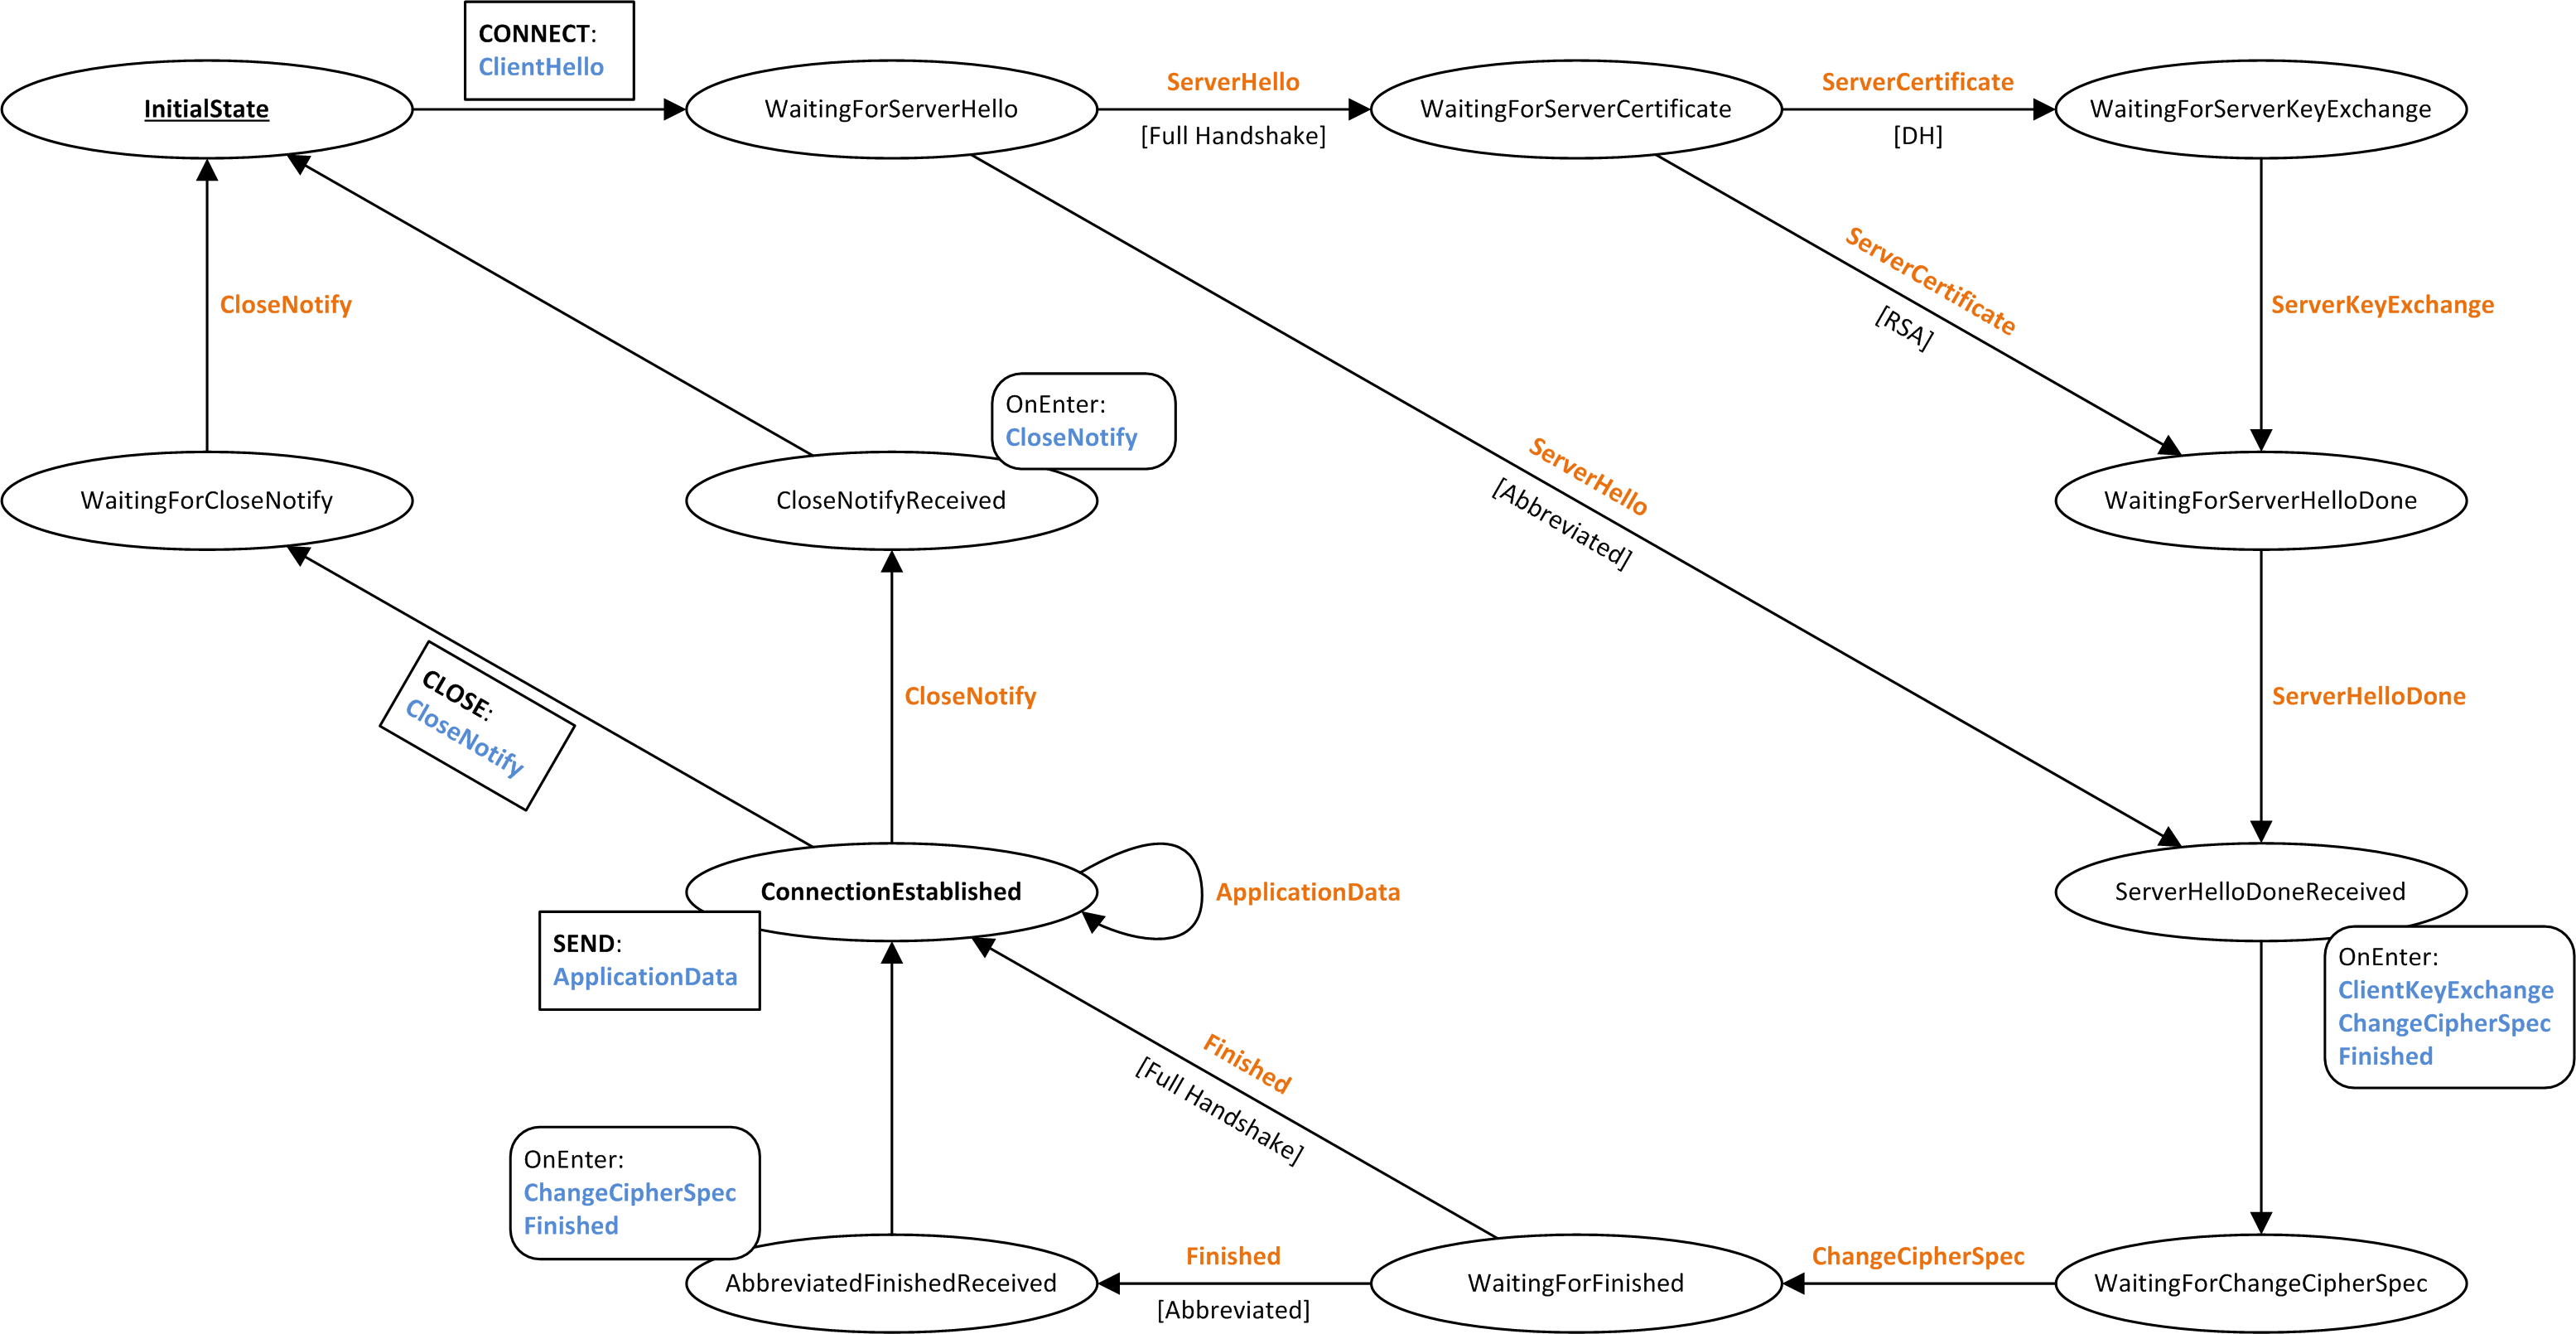
\includegraphics[scale=0.75, angle = 90]{Diagrams/client_state_machine.png} %
	\caption{Der Automat für den TLS-Client}
	\label{fig_tls_client_state_machine}
\end{figure}

\begin{figure}[H]
	\centering
	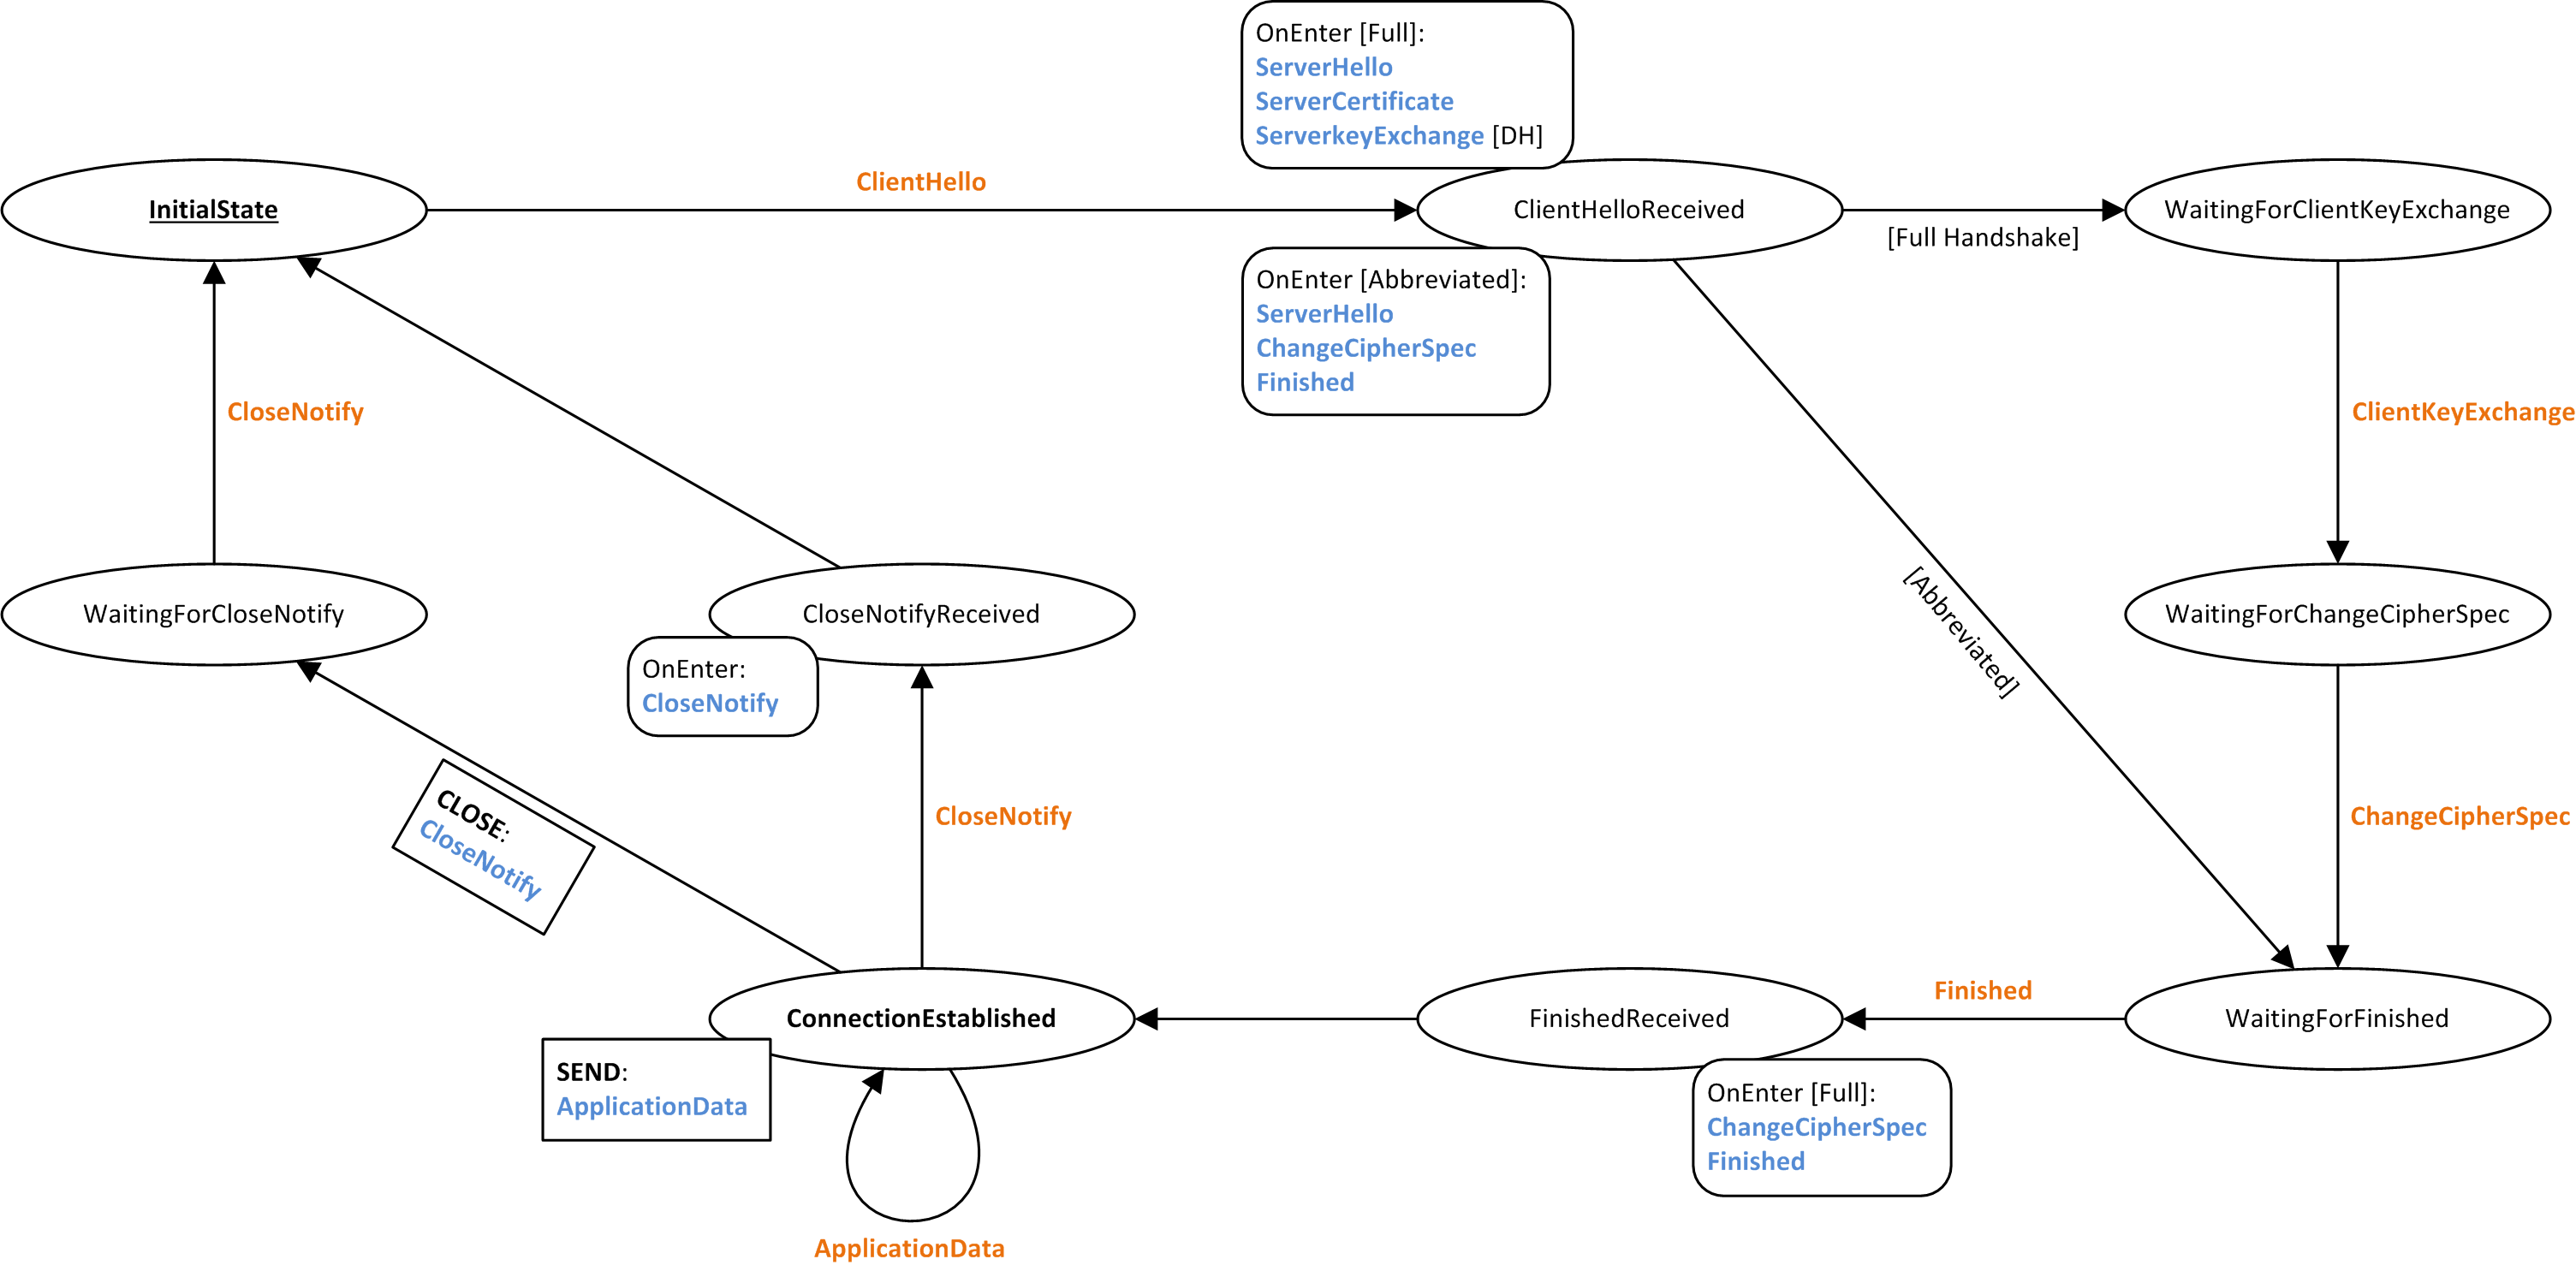
\includegraphics[scale=0.75, angle = 90]{Diagrams/server_state_machine.png} %
	\caption{Der Automat für den TLS-Server}
	\label{fig_tls_server_state_machine}
\end{figure}

\section{Tutorial: So schreibe ich ein Plugin, ...}


\appendix

\chapter{Fehlermeldungen des Alert Protocols}



\bibliography{quellen}
\bibliographystyle{alpha}

\listoftodos

\end{document}
